\documentclass[10pt]{report}
\usepackage{graphicx}
\parindent=0in
\textwidth=6.7in 
\textheight=9in
\setlength{\oddsidemargin}{-0.10in}
\setlength{\evensidemargin}{-0.10in}
\setlength{\topmargin}{-0.55in}
\setlength{\unitlength}{0.5in}
\pagestyle{empty}

\begin{document}

\begin{center}
{\large Instituto Tecnol\'{o}gico y de Estudios Superiores de Monterrey \\
An\'alisis Estad\'stico de Datos } \\
Examen Argumentativo (Papel)
\end{center}

Nombre: \underline{\hspace*{.2in}}
Keven Alexis Aispuro Bueno
\underline{\hspace*{.2in}} \quad Matr\'icula:\underline{\hspace*{.2in}}
A01743063
\underline{\hspace*{.2in}} \\

{\bf Instrucciones:} Lee con cuidado cada problema y escribe la soluci\'on
en tu hoja de respuesta. Incluye tu procedimiento que muestre c\'omo obtienes tu respuesta.  Respeta el c\'odigo de \'etica del curso y del Tecnol\'ogico de Monterrey y responde los ejercicios de manera individual sin ayuda externa o no autorizada.

\begin{enumerate}

\item Una empresa que fabrica l\'aminas de aluminio para la industria aeron\'autica necesita asegurar que el espesor de sus l\'aminas cumple con las especificaciones de $2.5 \pm 0.1$ mm. Se ha implementado una nueva maquinaria y se desea monitorear el espesor de las l\'aminas. Para ello, se han tomado muestras de tama\~no 5 cada hora y se gener\'o el diagrama que se muestra abajo.
\begin{enumerate}
\item (5 pts) Calcula la media y variabilidad del proceso (dentro de grupos).
\item (10 pts) Calcula los l\'imites de control para la {\bf variabilidad} del espesor de las láminas.
\item (10 pts) Calcula el porcentaje de l\'aminas que tienen un espesor menor a 2.4 mm. Use los valores del inciso a) para calcular este porcentaje.
\end{enumerate}
\begin{figure}[h!]
\centering
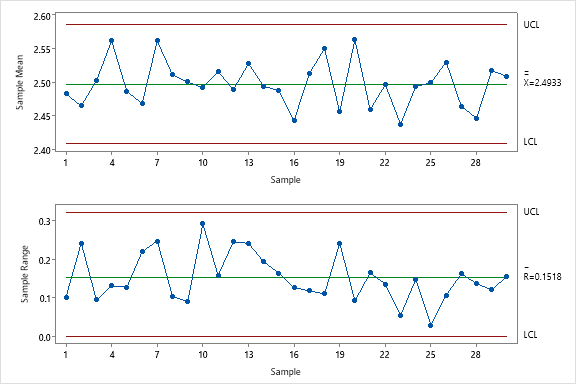
\includegraphics[width=0.75\textwidth]{Xbar_R_Paper.png}
\end{figure}


\item Una empresa que fabrica tarjetas de circuitos impresos desea evaluar si la implementaci\'on de un nuevo sistema de ensamblaje ha reducido el n\'umero de disconformidades. Se tomaron 50 mediciones, antes y después del cambio, para analizar los efectos.
\begin{center}
\begin{tabular}{|l|c|c|}
\hline
 & Antes & Después \\ 
\hline
Media muestral & 3.60 & 2.37 \\ 
\hline
Desviaci'on est'andar muestral & 1.09 & 1.62 \\ 
\hline
\end{tabular}
\end{center}
\begin{enumerate}
\item (15 pts) Calcula un intervalo de confianza de 90\% para el número medio de disconformidades antes del cambio.
\item (15 pts) Calcula un intervalo de confianza de 90\% para la estimar la diferencia en el número medio de disconformidades antes y después del cambio. ¿Qu\'e puedes concluir con este resultado?
\end{enumerate}


\end{enumerate}
  
\newpage



\begin{center}
{\large Instituto Tecnol\'{o}gico y de Estudios Superiores de Monterrey \\
An\'alisis Estad\'stico de Datos } \\
Examen Argumentativo (Papel)
\end{center}

Nombre: \underline{\hspace*{.2in}}
Rolando Araoz Borboa
\underline{\hspace*{.2in}} \quad Matr\'icula:\underline{\hspace*{.2in}}
A01741666
\underline{\hspace*{.2in}} \\

{\bf Instrucciones:} Lee con cuidado cada problema y escribe la soluci\'on
en tu hoja de respuesta. Incluye tu procedimiento que muestre c\'omo obtienes tu respuesta.  Respeta el c\'odigo de \'etica del curso y del Tecnol\'ogico de Monterrey y responde los ejercicios de manera individual sin ayuda externa o no autorizada.

\begin{enumerate}

\item Una empresa que fabrica l\'aminas de aluminio para la industria aeron\'autica necesita asegurar que el espesor de sus l\'aminas cumple con las especificaciones de $2.5 \pm 0.1$ mm. Se ha implementado una nueva maquinaria y se desea monitorear el espesor de las l\'aminas. Para ello, se han tomado muestras de tama\~no 4 cada hora y se gener\'o el diagrama que se muestra abajo.
\begin{enumerate}
\item (5 pts) Calcula la media y variabilidad del proceso (dentro de grupos).
\item (10 pts) Calcula los l\'imites de control para la {\bf variabilidad} del espesor de las láminas.
\item (10 pts) Calcula el porcentaje de l\'aminas que tienen un espesor mayor a 2.6 mm. Use los valores del inciso a) para calcular este porcentaje.
\end{enumerate}
\begin{figure}[h!]
\centering
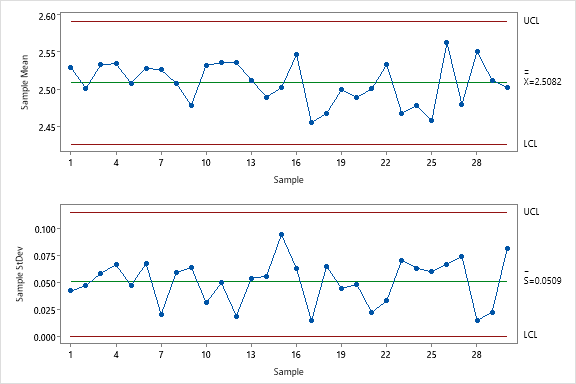
\includegraphics[width=0.75\textwidth]{Xbar_S_Paper.png}
\end{figure}


\item Una empresa que fabrica tarjetas de circuitos impresos desea evaluar si la implementaci\'on de un nuevo sistema de ensamblaje ha reducido el n\'umero de disconformidades. Se tomaron 50 mediciones, antes y después del cambio, para analizar los efectos.
\begin{center}
\begin{tabular}{|l|c|c|}
\hline
 & Antes & Después \\ 
\hline
Media muestral & 3.60 & 2.37 \\ 
\hline
Desviaci'on est'andar muestral & 1.09 & 1.62 \\ 
\hline
\end{tabular}
\end{center}
\begin{enumerate}
\item (15 pts) Calcula un intervalo de confianza de 90\% para el número medio de disconformidades antes del cambio.
\item (15 pts) ¿Existe suficiente evidencia para concluir que el número medio de disconformidades ha disminuido despu\'es del cambio? Usa un nivel de significancia de 0.05.
\end{enumerate}


\end{enumerate}
  
\newpage



\begin{center}
{\large Instituto Tecnol\'{o}gico y de Estudios Superiores de Monterrey \\
An\'alisis Estad\'stico de Datos } \\
Examen Argumentativo (Papel)
\end{center}

Nombre: \underline{\hspace*{.2in}}
Rodolfo Barron
\underline{\hspace*{.2in}} \quad Matr\'icula:\underline{\hspace*{.2in}}
A01741172
\underline{\hspace*{.2in}} \\

{\bf Instrucciones:} Lee con cuidado cada problema y escribe la soluci\'on
en tu hoja de respuesta. Incluye tu procedimiento que muestre c\'omo obtienes tu respuesta.  Respeta el c\'odigo de \'etica del curso y del Tecnol\'ogico de Monterrey y responde los ejercicios de manera individual sin ayuda externa o no autorizada.

\begin{enumerate}

\item Una empresa que fabrica l\'aminas de aluminio para la industria aeron\'autica necesita asegurar que el espesor de sus l\'aminas cumple con las especificaciones de $2.5 \pm 0.1$ mm. Se ha implementado una nueva maquinaria y se desea monitorear el espesor de las l\'aminas. Para ello, se han tomado muestras de tama\~no 5 cada hora y se gener\'o el diagrama que se muestra abajo.
\begin{enumerate}
\item (5 pts) Calcula la media y variabilidad del proceso (dentro de grupos).
\item (10 pts) Calcula los l\'imites de control para la {\bf variabilidad} del espesor de las láminas.
\item (10 pts) Calcula el porcentaje de l\'aminas que tienen un espesor menor a 2.4 mm. Use los valores del inciso a) para calcular este porcentaje.
\end{enumerate}
\begin{figure}[h!]
\centering
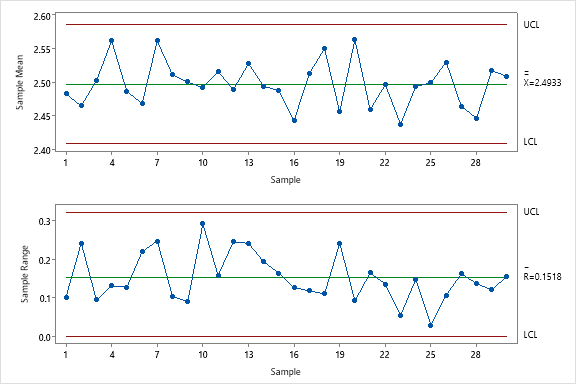
\includegraphics[width=0.75\textwidth]{Xbar_R_Paper.png}
\end{figure}


\item Una empresa que fabrica tarjetas de circuitos impresos desea evaluar si la implementaci\'on de un nuevo sistema de ensamblaje ha reducido el n\'umero de disconformidades. Se tomaron 50 mediciones, antes y después del cambio, para analizar los efectos.
\begin{center}
\begin{tabular}{|l|c|c|}
\hline
 & Antes & Después \\ 
\hline
Media muestral & 3.60 & 2.37 \\ 
\hline
Desviaci'on est'andar muestral & 1.09 & 1.62 \\ 
\hline
\end{tabular}
\end{center}
\begin{enumerate}
\item (15 pts) Calcula un intervalo de confianza de 90\% para el número medio de disconformidades antes del cambio.
\item (15 pts) Calcula un intervalo de confianza de 90\% para la estimar la diferencia en el número medio de disconformidades antes y después del cambio. ¿Qu\'e puedes concluir con este resultado?
\end{enumerate}


\end{enumerate}
  
\newpage



\begin{center}
{\large Instituto Tecnol\'{o}gico y de Estudios Superiores de Monterrey \\
An\'alisis Estad\'stico de Datos } \\
Examen Argumentativo (Papel)
\end{center}

Nombre: \underline{\hspace*{.2in}}
Danelle Bret\'on De Alba
\underline{\hspace*{.2in}} \quad Matr\'icula:\underline{\hspace*{.2in}}
A01741854
\underline{\hspace*{.2in}} \\

{\bf Instrucciones:} Lee con cuidado cada problema y escribe la soluci\'on
en tu hoja de respuesta. Incluye tu procedimiento que muestre c\'omo obtienes tu respuesta.  Respeta el c\'odigo de \'etica del curso y del Tecnol\'ogico de Monterrey y responde los ejercicios de manera individual sin ayuda externa o no autorizada.

\begin{enumerate}

\item Una empresa que fabrica l\'aminas de aluminio para la industria aeron\'autica necesita asegurar que el espesor de sus l\'aminas cumple con las especificaciones de $2.5 \pm 0.1$ mm. Se ha implementado una nueva maquinaria y se desea monitorear el espesor de las l\'aminas. Para ello, se han tomado muestras de tama\~no 4 cada hora y se gener\'o el diagrama que se muestra abajo.
\begin{enumerate}
\item (5 pts) Calcula la media y variabilidad del proceso (dentro de grupos).
\item (10 pts) Calcula los l\'imites de control para el espesor de las láminas.
\item (10 pts) Calcula el porcentaje de l\'aminas que cumplen con las especificaciones. Use los valores del inciso a) para calcular este porcentaje.
\end{enumerate}
\begin{figure}[h!]
\centering
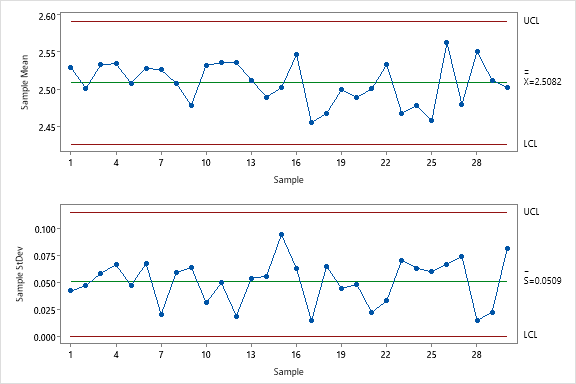
\includegraphics[width=0.75\textwidth]{Xbar_S_Paper.png}
\end{figure}


\item Una empresa que fabrica tarjetas de circuitos impresos desea evaluar si la implementaci\'on de un nuevo sistema de ensamblaje ha reducido el n\'umero de disconformidades. Se tomaron 50 mediciones, antes y después del cambio, para analizar los efectos.
\begin{center}
\begin{tabular}{|l|c|c|}
\hline
 & Antes & Después \\ 
\hline
Media muestral & 3.60 & 2.37 \\ 
\hline
Desviaci'on est'andar muestral & 1.09 & 1.62 \\ 
\hline
\end{tabular}
\end{center}
\begin{enumerate}
\item (15 pts) Calcula un intervalo de confianza de 90\% para el número medio de disconformidades antes del cambio.
\item (15 pts) Calcula un intervalo de confianza de 90\% para la estimar la diferencia en el número medio de disconformidades antes y después del cambio. ¿Qu\'e puedes concluir con este resultado?
\end{enumerate}


\end{enumerate}
  
\newpage



\begin{center}
{\large Instituto Tecnol\'{o}gico y de Estudios Superiores de Monterrey \\
An\'alisis Estad\'stico de Datos } \\
Examen Argumentativo (Papel)
\end{center}

Nombre: \underline{\hspace*{.2in}}
Sebastian Camacho Osuna
\underline{\hspace*{.2in}} \quad Matr\'icula:\underline{\hspace*{.2in}}
A01743160
\underline{\hspace*{.2in}} \\

{\bf Instrucciones:} Lee con cuidado cada problema y escribe la soluci\'on
en tu hoja de respuesta. Incluye tu procedimiento que muestre c\'omo obtienes tu respuesta.  Respeta el c\'odigo de \'etica del curso y del Tecnol\'ogico de Monterrey y responde los ejercicios de manera individual sin ayuda externa o no autorizada.

\begin{enumerate}

\item Una empresa que fabrica l\'aminas de aluminio para la industria aeron\'autica necesita asegurar que el espesor de sus l\'aminas cumple con las especificaciones de $2.5 \pm 0.1$ mm. Se ha implementado una nueva maquinaria y se desea monitorear el espesor de las l\'aminas. Para ello, se han tomado muestras de tama\~no 4 cada hora y se gener\'o el diagrama que se muestra abajo.
\begin{enumerate}
\item (5 pts) Calcula la media y variabilidad del proceso (dentro de grupos).
\item (10 pts) Calcula los l\'imites de control para el espesor de las láminas.
\item (10 pts) Calcula el porcentaje de l\'aminas que cumplen con las especificaciones. Use los valores del inciso a) para calcular este porcentaje.
\end{enumerate}
\begin{figure}[h!]
\centering
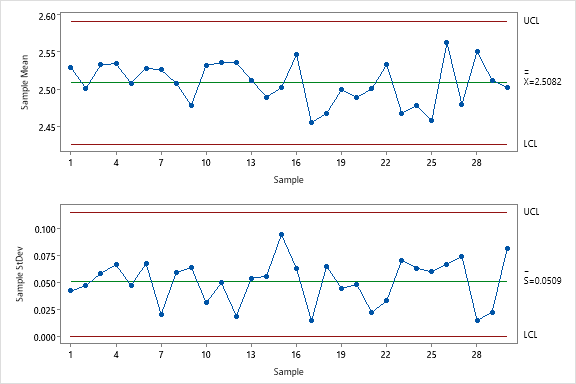
\includegraphics[width=0.75\textwidth]{Xbar_S_Paper.png}
\end{figure}


\item Una empresa que fabrica tarjetas de circuitos impresos desea evaluar si la implementaci\'on de un nuevo sistema de ensamblaje ha reducido el n\'umero de disconformidades. Se tomaron 50 mediciones, antes y después del cambio, para analizar los efectos.
\begin{center}
\begin{tabular}{|l|c|c|}
\hline
 & Antes & Después \\ 
\hline
Media muestral & 3.60 & 2.37 \\ 
\hline
Desviaci'on est'andar muestral & 1.09 & 1.62 \\ 
\hline
\end{tabular}
\end{center}
\begin{enumerate}
\item (15 pts) Calcula un intervalo de confianza de 90\% para el número medio de disconformidades antes del cambio.
\item (15 pts) ¿Existe suficiente evidencia para concluir que el número medio de disconformidades ha disminuido despu\'es del cambio? Usa un nivel de significancia de 0.05.
\end{enumerate}


\end{enumerate}
  
\newpage



\begin{center}
{\large Instituto Tecnol\'{o}gico y de Estudios Superiores de Monterrey \\
An\'alisis Estad\'stico de Datos } \\
Examen Argumentativo (Papel)
\end{center}

Nombre: \underline{\hspace*{.2in}}
Ahtziri Ceballos B\'aez
\underline{\hspace*{.2in}} \quad Matr\'icula:\underline{\hspace*{.2in}}
A01743247
\underline{\hspace*{.2in}} \\

{\bf Instrucciones:} Lee con cuidado cada problema y escribe la soluci\'on
en tu hoja de respuesta. Incluye tu procedimiento que muestre c\'omo obtienes tu respuesta.  Respeta el c\'odigo de \'etica del curso y del Tecnol\'ogico de Monterrey y responde los ejercicios de manera individual sin ayuda externa o no autorizada.

\begin{enumerate}

\item En una l\'inea de producci\'on de ejes para motores, el di\'ametro es una caracter\'istica crítica para el ensamblaje adecuado. Las especificaciones del di\'ametro son $50 \pm 0.5$ mm. Se mide el di\'ametro de un eje cada 30 minutos. Despu\'es de 15 horas de mediciones, se obtuvo el gr\'afico IMR con un promedio m\'ovil de orden 2 que se muestra abajo.
\begin{enumerate}
\item (5 pts) Calcula la media y variabilidad del proceso (dentro de grupos).
\item (10 pts) Calcula los l\'imites de control para el di\'ametro del eje.
\item (10 pts) Calcula el porcentaje de ejes que no cumplen con las especificaciones. Use los valores del inciso a) para calcular este porcentaje.
\end{enumerate}
\begin{figure}[h!]
\centering
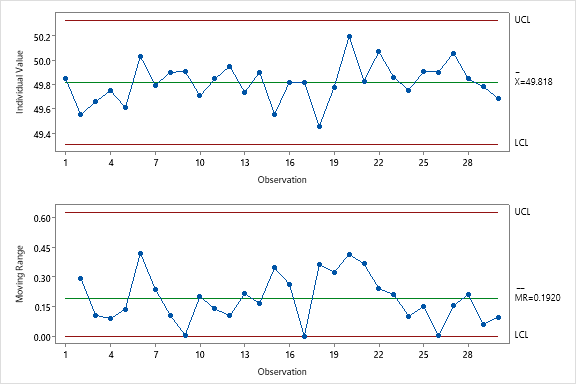
\includegraphics[width=0.75\textwidth]{IMR_Paper.png}
\end{figure}


\item Una empresa que fabrica tarjetas de circuitos impresos desea evaluar si la implementaci\'on de un nuevo sistema de ensamblaje ha reducido el n\'umero de disconformidades. Se tomaron 50 mediciones, antes y después del cambio, para analizar los efectos.
\begin{center}
\begin{tabular}{|l|c|c|}
\hline
 & Antes & Después \\ 
\hline
Media muestral & 3.60 & 2.37 \\ 
\hline
Desviaci'on est'andar muestral & 1.09 & 1.62 \\ 
\hline
\end{tabular}
\end{center}
\begin{enumerate}
\item (15 pts) Calcula un intervalo de confianza de 90\% para el número medio de disconformidades antes del cambio.
\item (15 pts) ¿Existe suficiente evidencia para concluir que el número medio de disconformidades ha disminuido despu\'es del cambio? Usa un nivel de significancia de 0.05.
\end{enumerate}


\end{enumerate}
  
\newpage



\begin{center}
{\large Instituto Tecnol\'{o}gico y de Estudios Superiores de Monterrey \\
An\'alisis Estad\'stico de Datos } \\
Examen Argumentativo (Papel)
\end{center}

Nombre: \underline{\hspace*{.2in}}
Ismael Alexander Cruz Lopez
\underline{\hspace*{.2in}} \quad Matr\'icula:\underline{\hspace*{.2in}}
A01743131
\underline{\hspace*{.2in}} \\

{\bf Instrucciones:} Lee con cuidado cada problema y escribe la soluci\'on
en tu hoja de respuesta. Incluye tu procedimiento que muestre c\'omo obtienes tu respuesta.  Respeta el c\'odigo de \'etica del curso y del Tecnol\'ogico de Monterrey y responde los ejercicios de manera individual sin ayuda externa o no autorizada.

\begin{enumerate}

\item Una empresa que fabrica l\'aminas de aluminio para la industria aeron\'autica necesita asegurar que el espesor de sus l\'aminas cumple con las especificaciones de $2.5 \pm 0.1$ mm. Se ha implementado una nueva maquinaria y se desea monitorear el espesor de las l\'aminas. Para ello, se han tomado muestras de tama\~no 4 cada hora y se gener\'o el diagrama que se muestra abajo.
\begin{enumerate}
\item (5 pts) Calcula la media y variabilidad del proceso (dentro de grupos).
\item (10 pts) Calcula los l\'imites de control para la {\bf variabilidad} del espesor de las láminas.
\item (10 pts) Calcula el porcentaje de l\'aminas que tienen un espesor mayor a 2.6 mm. Use los valores del inciso a) para calcular este porcentaje.
\end{enumerate}
\begin{figure}[h!]
\centering
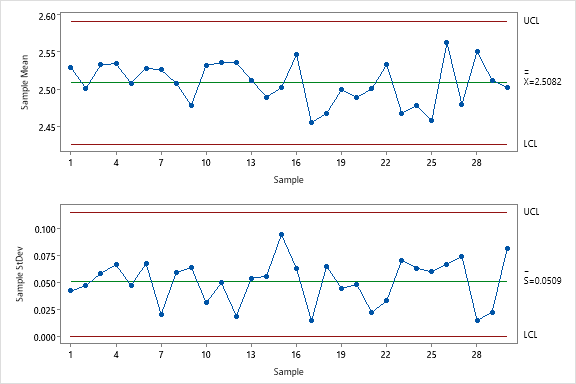
\includegraphics[width=0.75\textwidth]{Xbar_S_Paper.png}
\end{figure}


\item Una empresa que fabrica tarjetas de circuitos impresos desea evaluar si la implementaci\'on de un nuevo sistema de ensamblaje ha reducido el n\'umero de disconformidades. Se tomaron 50 mediciones, antes y después del cambio, para analizar los efectos.
\begin{center}
\begin{tabular}{|l|c|c|}
\hline
 & Antes & Después \\ 
\hline
Media muestral & 3.60 & 2.37 \\ 
\hline
Desviaci'on est'andar muestral & 1.09 & 1.62 \\ 
\hline
\end{tabular}
\end{center}
\begin{enumerate}
\item (15 pts) Calcula un intervalo de confianza de 90\% para el número medio de disconformidades antes del cambio.
\item (15 pts) ¿Existe suficiente evidencia para concluir que el número medio de disconformidades ha disminuido despu\'es del cambio? Usa un nivel de significancia de 0.05.
\end{enumerate}


\end{enumerate}
  
\newpage



\begin{center}
{\large Instituto Tecnol\'{o}gico y de Estudios Superiores de Monterrey \\
An\'alisis Estad\'stico de Datos } \\
Examen Argumentativo (Papel)
\end{center}

Nombre: \underline{\hspace*{.2in}}
Andr\'ee Espinoza Garnica
\underline{\hspace*{.2in}} \quad Matr\'icula:\underline{\hspace*{.2in}}
A01743134
\underline{\hspace*{.2in}} \\

{\bf Instrucciones:} Lee con cuidado cada problema y escribe la soluci\'on
en tu hoja de respuesta. Incluye tu procedimiento que muestre c\'omo obtienes tu respuesta.  Respeta el c\'odigo de \'etica del curso y del Tecnol\'ogico de Monterrey y responde los ejercicios de manera individual sin ayuda externa o no autorizada.

\begin{enumerate}

\item Una empresa que fabrica l\'aminas de aluminio para la industria aeron\'autica necesita asegurar que el espesor de sus l\'aminas cumple con las especificaciones de $2.5 \pm 0.1$ mm. Se ha implementado una nueva maquinaria y se desea monitorear el espesor de las l\'aminas. Para ello, se han tomado muestras de tama\~no 4 cada hora y se gener\'o el diagrama que se muestra abajo.
\begin{enumerate}
\item (5 pts) Calcula la media y variabilidad del proceso (dentro de grupos).
\item (10 pts) Calcula los l\'imites de control para el espesor de las láminas.
\item (10 pts) Calcula el porcentaje de l\'aminas que cumplen con las especificaciones. Use los valores del inciso a) para calcular este porcentaje.
\end{enumerate}
\begin{figure}[h!]
\centering
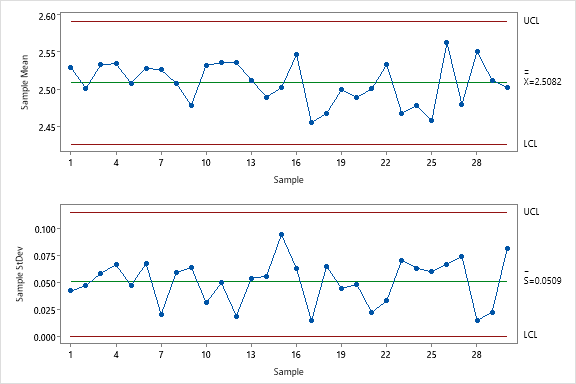
\includegraphics[width=0.75\textwidth]{Xbar_S_Paper.png}
\end{figure}


\item Una empresa que fabrica tarjetas de circuitos impresos desea evaluar si la implementaci\'on de un nuevo sistema de ensamblaje ha reducido el n\'umero de disconformidades. Se tomaron 50 mediciones, antes y después del cambio, para analizar los efectos.
\begin{center}
\begin{tabular}{|l|c|c|}
\hline
 & Antes & Después \\ 
\hline
Media muestral & 3.60 & 2.37 \\ 
\hline
Desviaci'on est'andar muestral & 1.09 & 1.62 \\ 
\hline
\end{tabular}
\end{center}
\begin{enumerate}
\item (15 pts) Calcula un intervalo de confianza de 90\% para el número medio de disconformidades antes del cambio.
\item (15 pts) ¿Existe suficiente evidencia para concluir que el número medio de disconformidades ha disminuido despu\'es del cambio? Usa un nivel de significancia de 0.05.
\end{enumerate}


\end{enumerate}
  
\newpage



\begin{center}
{\large Instituto Tecnol\'{o}gico y de Estudios Superiores de Monterrey \\
An\'alisis Estad\'stico de Datos } \\
Examen Argumentativo (Papel)
\end{center}

Nombre: \underline{\hspace*{.2in}}
Angel Paul Figueroa Flores
\underline{\hspace*{.2in}} \quad Matr\'icula:\underline{\hspace*{.2in}}
A01743218
\underline{\hspace*{.2in}} \\

{\bf Instrucciones:} Lee con cuidado cada problema y escribe la soluci\'on
en tu hoja de respuesta. Incluye tu procedimiento que muestre c\'omo obtienes tu respuesta.  Respeta el c\'odigo de \'etica del curso y del Tecnol\'ogico de Monterrey y responde los ejercicios de manera individual sin ayuda externa o no autorizada.

\begin{enumerate}

\item Una empresa que fabrica l\'aminas de aluminio para la industria aeron\'autica necesita asegurar que el espesor de sus l\'aminas cumple con las especificaciones de $2.5 \pm 0.1$ mm. Se ha implementado una nueva maquinaria y se desea monitorear el espesor de las l\'aminas. Para ello, se han tomado muestras de tama\~no 4 cada hora y se gener\'o el diagrama que se muestra abajo.
\begin{enumerate}
\item (5 pts) Calcula la media y variabilidad del proceso (dentro de grupos).
\item (10 pts) Calcula los l\'imites de control para la {\bf variabilidad} del espesor de las láminas.
\item (10 pts) Calcula el porcentaje de l\'aminas que tienen un espesor mayor a 2.6 mm. Use los valores del inciso a) para calcular este porcentaje.
\end{enumerate}
\begin{figure}[h!]
\centering
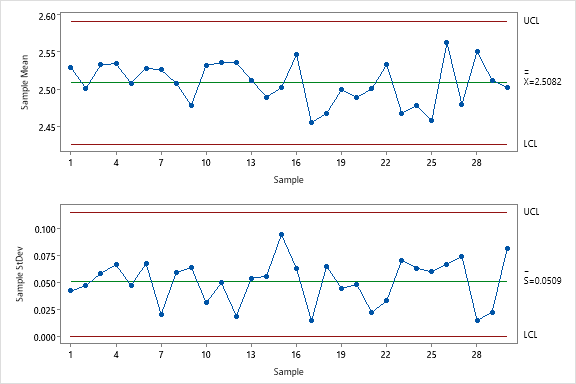
\includegraphics[width=0.75\textwidth]{Xbar_S_Paper.png}
\end{figure}


\item Una empresa que fabrica tarjetas de circuitos impresos desea evaluar si la implementaci\'on de un nuevo sistema de ensamblaje ha reducido el n\'umero de disconformidades. Se tomaron 50 mediciones, antes y después del cambio, para analizar los efectos.
\begin{center}
\begin{tabular}{|l|c|c|}
\hline
 & Antes & Después \\ 
\hline
Media muestral & 3.60 & 2.37 \\ 
\hline
Desviaci'on est'andar muestral & 1.09 & 1.62 \\ 
\hline
\end{tabular}
\end{center}
\begin{enumerate}
\item (15 pts) Calcula un intervalo de confianza de 90\% para el número medio de disconformidades antes del cambio.
\item (15 pts) Calcula un intervalo de confianza de 90\% para la estimar la diferencia en el número medio de disconformidades antes y después del cambio. ¿Qu\'e puedes concluir con este resultado?
\end{enumerate}


\end{enumerate}
  
\newpage



\begin{center}
{\large Instituto Tecnol\'{o}gico y de Estudios Superiores de Monterrey \\
An\'alisis Estad\'stico de Datos } \\
Examen Argumentativo (Papel)
\end{center}

Nombre: \underline{\hspace*{.2in}}
Rommel Federico Garc\'ia Pi\~na
\underline{\hspace*{.2in}} \quad Matr\'icula:\underline{\hspace*{.2in}}
A01743363
\underline{\hspace*{.2in}} \\

{\bf Instrucciones:} Lee con cuidado cada problema y escribe la soluci\'on
en tu hoja de respuesta. Incluye tu procedimiento que muestre c\'omo obtienes tu respuesta.  Respeta el c\'odigo de \'etica del curso y del Tecnol\'ogico de Monterrey y responde los ejercicios de manera individual sin ayuda externa o no autorizada.

\begin{enumerate}

\item Una empresa que fabrica l\'aminas de aluminio para la industria aeron\'autica necesita asegurar que el espesor de sus l\'aminas cumple con las especificaciones de $2.5 \pm 0.1$ mm. Se ha implementado una nueva maquinaria y se desea monitorear el espesor de las l\'aminas. Para ello, se han tomado muestras de tama\~no 4 cada hora y se gener\'o el diagrama que se muestra abajo.
\begin{enumerate}
\item (5 pts) Calcula la media y variabilidad del proceso (dentro de grupos).
\item (10 pts) Calcula los l\'imites de control para el espesor de las láminas.
\item (10 pts) Calcula el porcentaje de l\'aminas que cumplen con las especificaciones. Use los valores del inciso a) para calcular este porcentaje.
\end{enumerate}
\begin{figure}[h!]
\centering
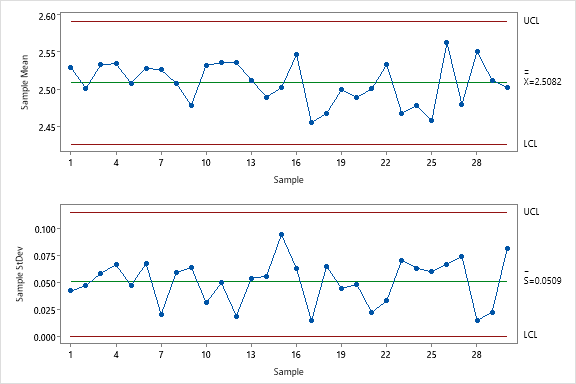
\includegraphics[width=0.75\textwidth]{Xbar_S_Paper.png}
\end{figure}


\item Una empresa que fabrica tarjetas de circuitos impresos desea evaluar si la implementaci\'on de un nuevo sistema de ensamblaje ha reducido el n\'umero de disconformidades. Se tomaron 50 mediciones, antes y después del cambio, para analizar los efectos.
\begin{center}
\begin{tabular}{|l|c|c|}
\hline
 & Antes & Después \\ 
\hline
Media muestral & 3.60 & 2.37 \\ 
\hline
Desviaci'on est'andar muestral & 1.09 & 1.62 \\ 
\hline
\end{tabular}
\end{center}
\begin{enumerate}
\item (15 pts) Calcula un intervalo de confianza de 90\% para el número medio de disconformidades antes del cambio.
\item (15 pts) Calcula un intervalo de confianza de 90\% para la estimar la diferencia en el número medio de disconformidades antes y después del cambio. ¿Qu\'e puedes concluir con este resultado?
\end{enumerate}


\end{enumerate}
  
\newpage



\begin{center}
{\large Instituto Tecnol\'{o}gico y de Estudios Superiores de Monterrey \\
An\'alisis Estad\'stico de Datos } \\
Examen Argumentativo (Papel)
\end{center}

Nombre: \underline{\hspace*{.2in}}
Jaime Eduardo Gast\'elum Castro
\underline{\hspace*{.2in}} \quad Matr\'icula:\underline{\hspace*{.2in}}
A01743071
\underline{\hspace*{.2in}} \\

{\bf Instrucciones:} Lee con cuidado cada problema y escribe la soluci\'on
en tu hoja de respuesta. Incluye tu procedimiento que muestre c\'omo obtienes tu respuesta.  Respeta el c\'odigo de \'etica del curso y del Tecnol\'ogico de Monterrey y responde los ejercicios de manera individual sin ayuda externa o no autorizada.

\begin{enumerate}

\item Una empresa que fabrica l\'aminas de aluminio para la industria aeron\'autica necesita asegurar que el espesor de sus l\'aminas cumple con las especificaciones de $2.5 \pm 0.1$ mm. Se ha implementado una nueva maquinaria y se desea monitorear el espesor de las l\'aminas. Para ello, se han tomado muestras de tama\~no 4 cada hora y se gener\'o el diagrama que se muestra abajo.
\begin{enumerate}
\item (5 pts) Calcula la media y variabilidad del proceso (dentro de grupos).
\item (10 pts) Calcula los l\'imites de control para la {\bf variabilidad} del espesor de las láminas.
\item (10 pts) Calcula el porcentaje de l\'aminas que tienen un espesor mayor a 2.6 mm. Use los valores del inciso a) para calcular este porcentaje.
\end{enumerate}
\begin{figure}[h!]
\centering
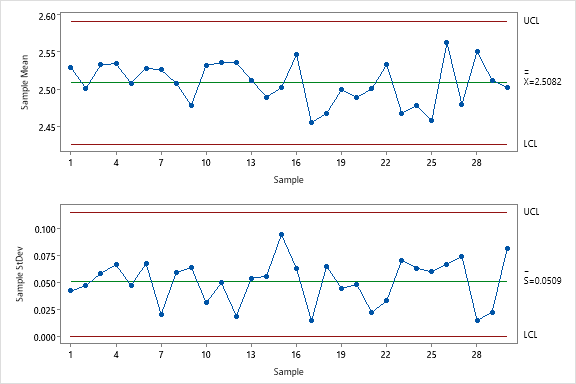
\includegraphics[width=0.75\textwidth]{Xbar_S_Paper.png}
\end{figure}


\item Una empresa que fabrica tarjetas de circuitos impresos desea evaluar si la implementaci\'on de un nuevo sistema de ensamblaje ha reducido el n\'umero de disconformidades. Se tomaron 50 mediciones, antes y después del cambio, para analizar los efectos.
\begin{center}
\begin{tabular}{|l|c|c|}
\hline
 & Antes & Después \\ 
\hline
Media muestral & 3.60 & 2.37 \\ 
\hline
Desviaci'on est'andar muestral & 1.09 & 1.62 \\ 
\hline
\end{tabular}
\end{center}
\begin{enumerate}
\item (15 pts) Calcula un intervalo de confianza de 90\% para el número medio de disconformidades antes del cambio.
\item (15 pts) ¿Existe suficiente evidencia para concluir que el número medio de disconformidades ha disminuido despu\'es del cambio? Usa un nivel de significancia de 0.05.
\end{enumerate}


\end{enumerate}
  
\newpage



\begin{center}
{\large Instituto Tecnol\'{o}gico y de Estudios Superiores de Monterrey \\
An\'alisis Estad\'stico de Datos } \\
Examen Argumentativo (Papel)
\end{center}

Nombre: \underline{\hspace*{.2in}}
Josué G\'omez Tirado
\underline{\hspace*{.2in}} \quad Matr\'icula:\underline{\hspace*{.2in}}
A00833429
\underline{\hspace*{.2in}} \\

{\bf Instrucciones:} Lee con cuidado cada problema y escribe la soluci\'on
en tu hoja de respuesta. Incluye tu procedimiento que muestre c\'omo obtienes tu respuesta.  Respeta el c\'odigo de \'etica del curso y del Tecnol\'ogico de Monterrey y responde los ejercicios de manera individual sin ayuda externa o no autorizada.

\begin{enumerate}

\item Una empresa que fabrica l\'aminas de aluminio para la industria aeron\'autica necesita asegurar que el espesor de sus l\'aminas cumple con las especificaciones de $2.5 \pm 0.1$ mm. Se ha implementado una nueva maquinaria y se desea monitorear el espesor de las l\'aminas. Para ello, se han tomado muestras de tama\~no 5 cada hora y se gener\'o el diagrama que se muestra abajo.
\begin{enumerate}
\item (5 pts) Calcula la media y variabilidad del proceso (dentro de grupos).
\item (10 pts) Calcula los l\'imites de control para la {\bf variabilidad} del espesor de las láminas.
\item (10 pts) Calcula el porcentaje de l\'aminas que tienen un espesor menor a 2.4 mm. Use los valores del inciso a) para calcular este porcentaje.
\end{enumerate}
\begin{figure}[h!]
\centering
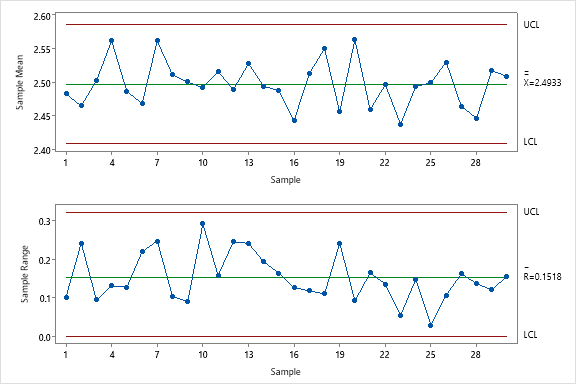
\includegraphics[width=0.75\textwidth]{Xbar_R_Paper.png}
\end{figure}


\item Una empresa que fabrica tarjetas de circuitos impresos desea evaluar si la implementaci\'on de un nuevo sistema de ensamblaje ha reducido el n\'umero de disconformidades. Se tomaron 50 mediciones, antes y después del cambio, para analizar los efectos.
\begin{center}
\begin{tabular}{|l|c|c|}
\hline
 & Antes & Después \\ 
\hline
Media muestral & 3.60 & 2.37 \\ 
\hline
Desviaci'on est'andar muestral & 1.09 & 1.62 \\ 
\hline
\end{tabular}
\end{center}
\begin{enumerate}
\item (15 pts) Calcula un intervalo de confianza de 90\% para el número medio de disconformidades antes del cambio.
\item (15 pts) ¿Existe suficiente evidencia para concluir que el número medio de disconformidades ha disminuido despu\'es del cambio? Usa un nivel de significancia de 0.05.
\end{enumerate}


\end{enumerate}
  
\newpage



\begin{center}
{\large Instituto Tecnol\'{o}gico y de Estudios Superiores de Monterrey \\
An\'alisis Estad\'stico de Datos } \\
Examen Argumentativo (Papel)
\end{center}

Nombre: \underline{\hspace*{.2in}}
Carmen Mar\'ia Heras Mu\~noz
\underline{\hspace*{.2in}} \quad Matr\'icula:\underline{\hspace*{.2in}}
A01742526
\underline{\hspace*{.2in}} \\

{\bf Instrucciones:} Lee con cuidado cada problema y escribe la soluci\'on
en tu hoja de respuesta. Incluye tu procedimiento que muestre c\'omo obtienes tu respuesta.  Respeta el c\'odigo de \'etica del curso y del Tecnol\'ogico de Monterrey y responde los ejercicios de manera individual sin ayuda externa o no autorizada.

\begin{enumerate}

\item En una l\'inea de producci\'on de ejes para motores, el di\'ametro es una caracter\'istica crítica para el ensamblaje adecuado. Las especificaciones del di\'ametro son $50 \pm 0.5$ mm. Se mide el di\'ametro de un eje cada 30 minutos. Despu\'es de 15 horas de mediciones, se obtuvo el gr\'afico IMR con un promedio m\'ovil de orden 2 que se muestra abajo.
\begin{enumerate}
\item (5 pts) Calcula la media y variabilidad del proceso (dentro de grupos).
\item (10 pts) Calcula los l\'imites de control para el di\'ametro del eje.
\item (10 pts) Calcula el porcentaje de ejes que no cumplen con las especificaciones. Use los valores del inciso a) para calcular este porcentaje.
\end{enumerate}
\begin{figure}[h!]
\centering
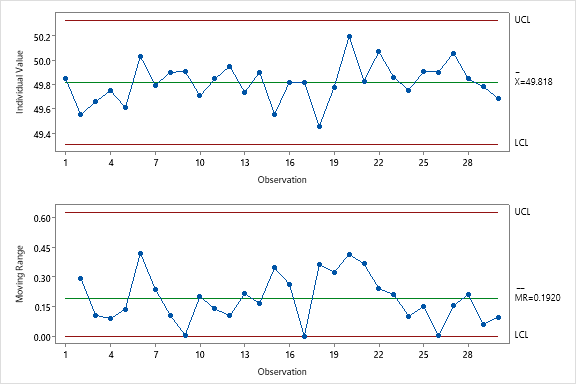
\includegraphics[width=0.75\textwidth]{IMR_Paper.png}
\end{figure}


\item Una empresa que fabrica tarjetas de circuitos impresos desea evaluar si la implementaci\'on de un nuevo sistema de ensamblaje ha reducido el n\'umero de disconformidades. Se tomaron 50 mediciones, antes y después del cambio, para analizar los efectos.
\begin{center}
\begin{tabular}{|l|c|c|}
\hline
 & Antes & Después \\ 
\hline
Media muestral & 3.60 & 2.37 \\ 
\hline
Desviaci'on est'andar muestral & 1.09 & 1.62 \\ 
\hline
\end{tabular}
\end{center}
\begin{enumerate}
\item (15 pts) Calcula un intervalo de confianza de 90\% para el número medio de disconformidades antes del cambio.
\item (15 pts) ¿Existe suficiente evidencia para concluir que el número medio de disconformidades ha disminuido despu\'es del cambio? Usa un nivel de significancia de 0.05.
\end{enumerate}


\end{enumerate}
  
\newpage



\begin{center}
{\large Instituto Tecnol\'{o}gico y de Estudios Superiores de Monterrey \\
An\'alisis Estad\'stico de Datos } \\
Examen Argumentativo (Papel)
\end{center}

Nombre: \underline{\hspace*{.2in}}
Carlos Hermosillo Berrelleza
\underline{\hspace*{.2in}} \quad Matr\'icula:\underline{\hspace*{.2in}}
A01741829
\underline{\hspace*{.2in}} \\

{\bf Instrucciones:} Lee con cuidado cada problema y escribe la soluci\'on
en tu hoja de respuesta. Incluye tu procedimiento que muestre c\'omo obtienes tu respuesta.  Respeta el c\'odigo de \'etica del curso y del Tecnol\'ogico de Monterrey y responde los ejercicios de manera individual sin ayuda externa o no autorizada.

\begin{enumerate}

\item Una empresa que fabrica l\'aminas de aluminio para la industria aeron\'autica necesita asegurar que el espesor de sus l\'aminas cumple con las especificaciones de $2.5 \pm 0.1$ mm. Se ha implementado una nueva maquinaria y se desea monitorear el espesor de las l\'aminas. Para ello, se han tomado muestras de tama\~no 5 cada hora y se gener\'o el diagrama que se muestra abajo.
\begin{enumerate}
\item (5 pts) Calcula la media y variabilidad del proceso (dentro de grupos).
\item (10 pts) Calcula los l\'imites de control para el espesor de las láminas.
\item (10 pts) Calcula el porcentaje de l\'aminas que no cumplen con las especificaciones. Use los valores del inciso a) para calcular este porcentaje.
\end{enumerate}
\begin{figure}[h!]
\centering
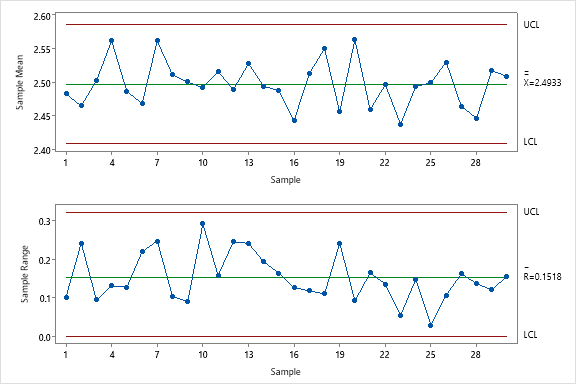
\includegraphics[width=0.75\textwidth]{Xbar_R_Paper.png}
\end{figure}


\item Una empresa que fabrica tarjetas de circuitos impresos desea evaluar si la implementaci\'on de un nuevo sistema de ensamblaje ha reducido el n\'umero de disconformidades. Se tomaron 50 mediciones, antes y después del cambio, para analizar los efectos.
\begin{center}
\begin{tabular}{|l|c|c|}
\hline
 & Antes & Después \\ 
\hline
Media muestral & 3.60 & 2.37 \\ 
\hline
Desviaci'on est'andar muestral & 1.09 & 1.62 \\ 
\hline
\end{tabular}
\end{center}
\begin{enumerate}
\item (15 pts) Calcula un intervalo de confianza de 90\% para el número medio de disconformidades antes del cambio.
\item (15 pts) Calcula un intervalo de confianza de 90\% para la estimar la diferencia en el número medio de disconformidades antes y después del cambio. ¿Qu\'e puedes concluir con este resultado?
\end{enumerate}


\end{enumerate}
  
\newpage



\begin{center}
{\large Instituto Tecnol\'{o}gico y de Estudios Superiores de Monterrey \\
An\'alisis Estad\'stico de Datos } \\
Examen Argumentativo (Papel)
\end{center}

Nombre: \underline{\hspace*{.2in}}
Alejandro Ibarra Espinoza
\underline{\hspace*{.2in}} \quad Matr\'icula:\underline{\hspace*{.2in}}
A01743290
\underline{\hspace*{.2in}} \\

{\bf Instrucciones:} Lee con cuidado cada problema y escribe la soluci\'on
en tu hoja de respuesta. Incluye tu procedimiento que muestre c\'omo obtienes tu respuesta.  Respeta el c\'odigo de \'etica del curso y del Tecnol\'ogico de Monterrey y responde los ejercicios de manera individual sin ayuda externa o no autorizada.

\begin{enumerate}

\item Una empresa que fabrica l\'aminas de aluminio para la industria aeron\'autica necesita asegurar que el espesor de sus l\'aminas cumple con las especificaciones de $2.5 \pm 0.1$ mm. Se ha implementado una nueva maquinaria y se desea monitorear el espesor de las l\'aminas. Para ello, se han tomado muestras de tama\~no 4 cada hora y se gener\'o el diagrama que se muestra abajo.
\begin{enumerate}
\item (5 pts) Calcula la media y variabilidad del proceso (dentro de grupos).
\item (10 pts) Calcula los l\'imites de control para el espesor de las láminas.
\item (10 pts) Calcula el porcentaje de l\'aminas que cumplen con las especificaciones. Use los valores del inciso a) para calcular este porcentaje.
\end{enumerate}
\begin{figure}[h!]
\centering
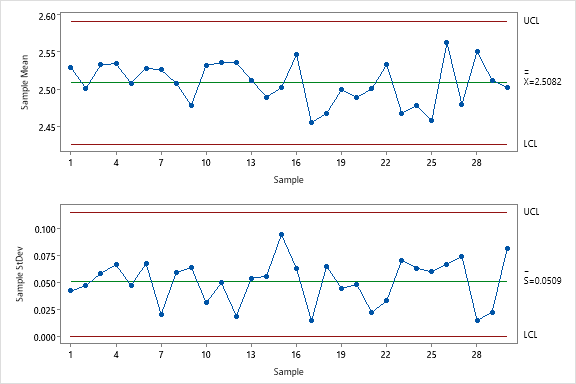
\includegraphics[width=0.75\textwidth]{Xbar_S_Paper.png}
\end{figure}


\item Una empresa que fabrica tarjetas de circuitos impresos desea evaluar si la implementaci\'on de un nuevo sistema de ensamblaje ha reducido el n\'umero de disconformidades. Se tomaron 50 mediciones, antes y después del cambio, para analizar los efectos.
\begin{center}
\begin{tabular}{|l|c|c|}
\hline
 & Antes & Después \\ 
\hline
Media muestral & 3.60 & 2.37 \\ 
\hline
Desviaci'on est'andar muestral & 1.09 & 1.62 \\ 
\hline
\end{tabular}
\end{center}
\begin{enumerate}
\item (15 pts) Calcula un intervalo de confianza de 90\% para el número medio de disconformidades antes del cambio.
\item (15 pts) ¿Existe suficiente evidencia para concluir que el número medio de disconformidades ha disminuido despu\'es del cambio? Usa un nivel de significancia de 0.05.
\end{enumerate}


\end{enumerate}
  
\newpage



\begin{center}
{\large Instituto Tecnol\'{o}gico y de Estudios Superiores de Monterrey \\
An\'alisis Estad\'stico de Datos } \\
Examen Argumentativo (Papel)
\end{center}

Nombre: \underline{\hspace*{.2in}}
Montserrat Ibarra S\'anchez
\underline{\hspace*{.2in}} \quad Matr\'icula:\underline{\hspace*{.2in}}
A01741649
\underline{\hspace*{.2in}} \\

{\bf Instrucciones:} Lee con cuidado cada problema y escribe la soluci\'on
en tu hoja de respuesta. Incluye tu procedimiento que muestre c\'omo obtienes tu respuesta.  Respeta el c\'odigo de \'etica del curso y del Tecnol\'ogico de Monterrey y responde los ejercicios de manera individual sin ayuda externa o no autorizada.

\begin{enumerate}

\item Una empresa que fabrica l\'aminas de aluminio para la industria aeron\'autica necesita asegurar que el espesor de sus l\'aminas cumple con las especificaciones de $2.5 \pm 0.1$ mm. Se ha implementado una nueva maquinaria y se desea monitorear el espesor de las l\'aminas. Para ello, se han tomado muestras de tama\~no 4 cada hora y se gener\'o el diagrama que se muestra abajo.
\begin{enumerate}
\item (5 pts) Calcula la media y variabilidad del proceso (dentro de grupos).
\item (10 pts) Calcula los l\'imites de control para el espesor de las láminas.
\item (10 pts) Calcula el porcentaje de l\'aminas que cumplen con las especificaciones. Use los valores del inciso a) para calcular este porcentaje.
\end{enumerate}
\begin{figure}[h!]
\centering
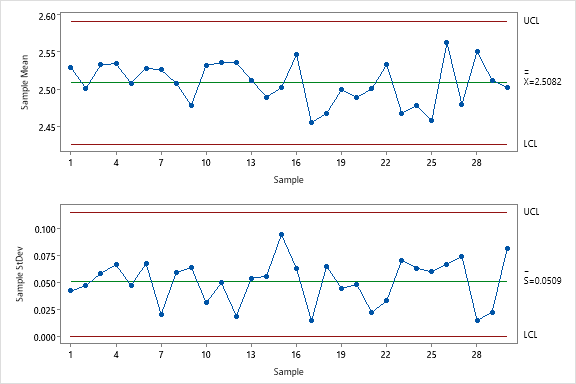
\includegraphics[width=0.75\textwidth]{Xbar_S_Paper.png}
\end{figure}


\item Una empresa que fabrica tarjetas de circuitos impresos desea evaluar si la implementaci\'on de un nuevo sistema de ensamblaje ha reducido el n\'umero de disconformidades. Se tomaron 50 mediciones, antes y después del cambio, para analizar los efectos.
\begin{center}
\begin{tabular}{|l|c|c|}
\hline
 & Antes & Después \\ 
\hline
Media muestral & 3.60 & 2.37 \\ 
\hline
Desviaci'on est'andar muestral & 1.09 & 1.62 \\ 
\hline
\end{tabular}
\end{center}
\begin{enumerate}
\item (15 pts) Calcula un intervalo de confianza de 90\% para el número medio de disconformidades antes del cambio.
\item (15 pts) Calcula un intervalo de confianza de 90\% para la estimar la diferencia en el número medio de disconformidades antes y después del cambio. ¿Qu\'e puedes concluir con este resultado?
\end{enumerate}


\end{enumerate}
  
\newpage



\begin{center}
{\large Instituto Tecnol\'{o}gico y de Estudios Superiores de Monterrey \\
An\'alisis Estad\'stico de Datos } \\
Examen Argumentativo (Papel)
\end{center}

Nombre: \underline{\hspace*{.2in}}
Gerardo Lozano Gallardo
\underline{\hspace*{.2in}} \quad Matr\'icula:\underline{\hspace*{.2in}}
A01742948
\underline{\hspace*{.2in}} \\

{\bf Instrucciones:} Lee con cuidado cada problema y escribe la soluci\'on
en tu hoja de respuesta. Incluye tu procedimiento que muestre c\'omo obtienes tu respuesta.  Respeta el c\'odigo de \'etica del curso y del Tecnol\'ogico de Monterrey y responde los ejercicios de manera individual sin ayuda externa o no autorizada.

\begin{enumerate}

\item Una empresa que fabrica l\'aminas de aluminio para la industria aeron\'autica necesita asegurar que el espesor de sus l\'aminas cumple con las especificaciones de $2.5 \pm 0.1$ mm. Se ha implementado una nueva maquinaria y se desea monitorear el espesor de las l\'aminas. Para ello, se han tomado muestras de tama\~no 5 cada hora y se gener\'o el diagrama que se muestra abajo.
\begin{enumerate}
\item (5 pts) Calcula la media y variabilidad del proceso (dentro de grupos).
\item (10 pts) Calcula los l\'imites de control para la {\bf variabilidad} del espesor de las láminas.
\item (10 pts) Calcula el porcentaje de l\'aminas que tienen un espesor menor a 2.4 mm. Use los valores del inciso a) para calcular este porcentaje.
\end{enumerate}
\begin{figure}[h!]
\centering
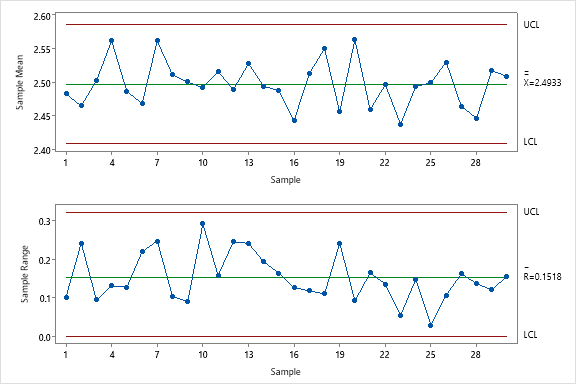
\includegraphics[width=0.75\textwidth]{Xbar_R_Paper.png}
\end{figure}


\item Una empresa que fabrica tarjetas de circuitos impresos desea evaluar si la implementaci\'on de un nuevo sistema de ensamblaje ha reducido el n\'umero de disconformidades. Se tomaron 50 mediciones, antes y después del cambio, para analizar los efectos.
\begin{center}
\begin{tabular}{|l|c|c|}
\hline
 & Antes & Después \\ 
\hline
Media muestral & 3.60 & 2.37 \\ 
\hline
Desviaci'on est'andar muestral & 1.09 & 1.62 \\ 
\hline
\end{tabular}
\end{center}
\begin{enumerate}
\item (15 pts) Calcula un intervalo de confianza de 90\% para el número medio de disconformidades antes del cambio.
\item (15 pts) Calcula un intervalo de confianza de 90\% para la estimar la diferencia en el número medio de disconformidades antes y después del cambio. ¿Qu\'e puedes concluir con este resultado?
\end{enumerate}


\end{enumerate}
  
\newpage



\begin{center}
{\large Instituto Tecnol\'{o}gico y de Estudios Superiores de Monterrey \\
An\'alisis Estad\'stico de Datos } \\
Examen Argumentativo (Papel)
\end{center}

Nombre: \underline{\hspace*{.2in}}
Romina Luna Herrera
\underline{\hspace*{.2in}} \quad Matr\'icula:\underline{\hspace*{.2in}}
A01743206
\underline{\hspace*{.2in}} \\

{\bf Instrucciones:} Lee con cuidado cada problema y escribe la soluci\'on
en tu hoja de respuesta. Incluye tu procedimiento que muestre c\'omo obtienes tu respuesta.  Respeta el c\'odigo de \'etica del curso y del Tecnol\'ogico de Monterrey y responde los ejercicios de manera individual sin ayuda externa o no autorizada.

\begin{enumerate}

\item Una empresa que fabrica l\'aminas de aluminio para la industria aeron\'autica necesita asegurar que el espesor de sus l\'aminas cumple con las especificaciones de $2.5 \pm 0.1$ mm. Se ha implementado una nueva maquinaria y se desea monitorear el espesor de las l\'aminas. Para ello, se han tomado muestras de tama\~no 4 cada hora y se gener\'o el diagrama que se muestra abajo.
\begin{enumerate}
\item (5 pts) Calcula la media y variabilidad del proceso (dentro de grupos).
\item (10 pts) Calcula los l\'imites de control para el espesor de las láminas.
\item (10 pts) Calcula el porcentaje de l\'aminas que cumplen con las especificaciones. Use los valores del inciso a) para calcular este porcentaje.
\end{enumerate}
\begin{figure}[h!]
\centering
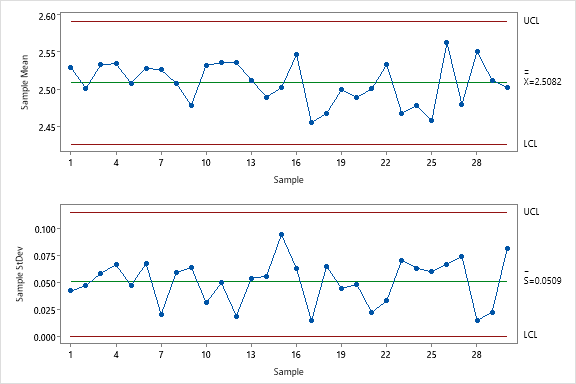
\includegraphics[width=0.75\textwidth]{Xbar_S_Paper.png}
\end{figure}


\item Una empresa que fabrica tarjetas de circuitos impresos desea evaluar si la implementaci\'on de un nuevo sistema de ensamblaje ha reducido el n\'umero de disconformidades. Se tomaron 50 mediciones, antes y después del cambio, para analizar los efectos.
\begin{center}
\begin{tabular}{|l|c|c|}
\hline
 & Antes & Después \\ 
\hline
Media muestral & 3.60 & 2.37 \\ 
\hline
Desviaci'on est'andar muestral & 1.09 & 1.62 \\ 
\hline
\end{tabular}
\end{center}
\begin{enumerate}
\item (15 pts) Calcula un intervalo de confianza de 90\% para el número medio de disconformidades antes del cambio.
\item (15 pts) ¿Existe suficiente evidencia para concluir que el número medio de disconformidades ha disminuido despu\'es del cambio? Usa un nivel de significancia de 0.05.
\end{enumerate}


\end{enumerate}
  
\newpage



\begin{center}
{\large Instituto Tecnol\'{o}gico y de Estudios Superiores de Monterrey \\
An\'alisis Estad\'stico de Datos } \\
Examen Argumentativo (Papel)
\end{center}

Nombre: \underline{\hspace*{.2in}}
Eduardo Madrigal V\'azquez
\underline{\hspace*{.2in}} \quad Matr\'icula:\underline{\hspace*{.2in}}
A01742934
\underline{\hspace*{.2in}} \\

{\bf Instrucciones:} Lee con cuidado cada problema y escribe la soluci\'on
en tu hoja de respuesta. Incluye tu procedimiento que muestre c\'omo obtienes tu respuesta.  Respeta el c\'odigo de \'etica del curso y del Tecnol\'ogico de Monterrey y responde los ejercicios de manera individual sin ayuda externa o no autorizada.

\begin{enumerate}

\item Una empresa que fabrica l\'aminas de aluminio para la industria aeron\'autica necesita asegurar que el espesor de sus l\'aminas cumple con las especificaciones de $2.5 \pm 0.1$ mm. Se ha implementado una nueva maquinaria y se desea monitorear el espesor de las l\'aminas. Para ello, se han tomado muestras de tama\~no 5 cada hora y se gener\'o el diagrama que se muestra abajo.
\begin{enumerate}
\item (5 pts) Calcula la media y variabilidad del proceso (dentro de grupos).
\item (10 pts) Calcula los l\'imites de control para la {\bf variabilidad} del espesor de las láminas.
\item (10 pts) Calcula el porcentaje de l\'aminas que tienen un espesor menor a 2.4 mm. Use los valores del inciso a) para calcular este porcentaje.
\end{enumerate}
\begin{figure}[h!]
\centering
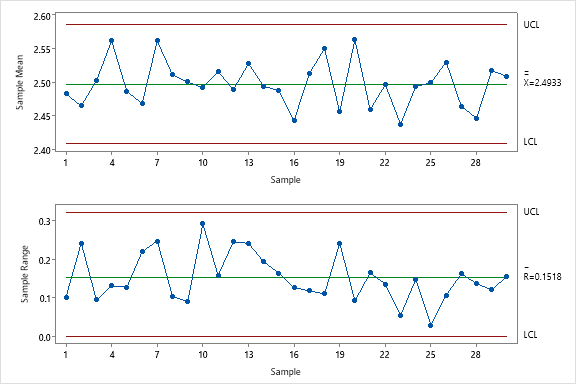
\includegraphics[width=0.75\textwidth]{Xbar_R_Paper.png}
\end{figure}


\item Una empresa que fabrica tarjetas de circuitos impresos desea evaluar si la implementaci\'on de un nuevo sistema de ensamblaje ha reducido el n\'umero de disconformidades. Se tomaron 50 mediciones, antes y después del cambio, para analizar los efectos.
\begin{center}
\begin{tabular}{|l|c|c|}
\hline
 & Antes & Después \\ 
\hline
Media muestral & 3.60 & 2.37 \\ 
\hline
Desviaci'on est'andar muestral & 1.09 & 1.62 \\ 
\hline
\end{tabular}
\end{center}
\begin{enumerate}
\item (15 pts) Calcula un intervalo de confianza de 90\% para el número medio de disconformidades antes del cambio.
\item (15 pts) ¿Existe suficiente evidencia para concluir que el número medio de disconformidades ha disminuido despu\'es del cambio? Usa un nivel de significancia de 0.05.
\end{enumerate}


\end{enumerate}
  
\newpage



\begin{center}
{\large Instituto Tecnol\'{o}gico y de Estudios Superiores de Monterrey \\
An\'alisis Estad\'stico de Datos } \\
Examen Argumentativo (Papel)
\end{center}

Nombre: \underline{\hspace*{.2in}}
Usiel Josu\'e Mart\'inez Calvo
\underline{\hspace*{.2in}} \quad Matr\'icula:\underline{\hspace*{.2in}}
A01742937
\underline{\hspace*{.2in}} \\

{\bf Instrucciones:} Lee con cuidado cada problema y escribe la soluci\'on
en tu hoja de respuesta. Incluye tu procedimiento que muestre c\'omo obtienes tu respuesta.  Respeta el c\'odigo de \'etica del curso y del Tecnol\'ogico de Monterrey y responde los ejercicios de manera individual sin ayuda externa o no autorizada.

\begin{enumerate}

\item Una empresa que fabrica l\'aminas de aluminio para la industria aeron\'autica necesita asegurar que el espesor de sus l\'aminas cumple con las especificaciones de $2.5 \pm 0.1$ mm. Se ha implementado una nueva maquinaria y se desea monitorear el espesor de las l\'aminas. Para ello, se han tomado muestras de tama\~no 5 cada hora y se gener\'o el diagrama que se muestra abajo.
\begin{enumerate}
\item (5 pts) Calcula la media y variabilidad del proceso (dentro de grupos).
\item (10 pts) Calcula los l\'imites de control para el espesor de las láminas.
\item (10 pts) Calcula el porcentaje de l\'aminas que no cumplen con las especificaciones. Use los valores del inciso a) para calcular este porcentaje.
\end{enumerate}
\begin{figure}[h!]
\centering
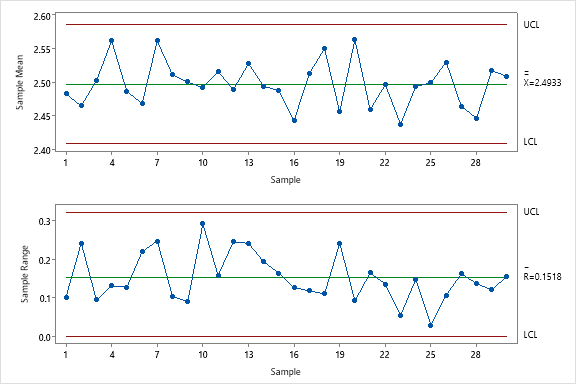
\includegraphics[width=0.75\textwidth]{Xbar_R_Paper.png}
\end{figure}


\item Una empresa que fabrica tarjetas de circuitos impresos desea evaluar si la implementaci\'on de un nuevo sistema de ensamblaje ha reducido el n\'umero de disconformidades. Se tomaron 50 mediciones, antes y después del cambio, para analizar los efectos.
\begin{center}
\begin{tabular}{|l|c|c|}
\hline
 & Antes & Después \\ 
\hline
Media muestral & 3.60 & 2.37 \\ 
\hline
Desviaci'on est'andar muestral & 1.09 & 1.62 \\ 
\hline
\end{tabular}
\end{center}
\begin{enumerate}
\item (15 pts) Calcula un intervalo de confianza de 90\% para el número medio de disconformidades antes del cambio.
\item (15 pts) ¿Existe suficiente evidencia para concluir que el número medio de disconformidades ha disminuido despu\'es del cambio? Usa un nivel de significancia de 0.05.
\end{enumerate}


\end{enumerate}
  
\newpage



\begin{center}
{\large Instituto Tecnol\'{o}gico y de Estudios Superiores de Monterrey \\
An\'alisis Estad\'stico de Datos } \\
Examen Argumentativo (Papel)
\end{center}

Nombre: \underline{\hspace*{.2in}}
Gerardo Medina Santiago
\underline{\hspace*{.2in}} \quad Matr\'icula:\underline{\hspace*{.2in}}
A01741230
\underline{\hspace*{.2in}} \\

{\bf Instrucciones:} Lee con cuidado cada problema y escribe la soluci\'on
en tu hoja de respuesta. Incluye tu procedimiento que muestre c\'omo obtienes tu respuesta.  Respeta el c\'odigo de \'etica del curso y del Tecnol\'ogico de Monterrey y responde los ejercicios de manera individual sin ayuda externa o no autorizada.

\begin{enumerate}

\item Una empresa que fabrica l\'aminas de aluminio para la industria aeron\'autica necesita asegurar que el espesor de sus l\'aminas cumple con las especificaciones de $2.5 \pm 0.1$ mm. Se ha implementado una nueva maquinaria y se desea monitorear el espesor de las l\'aminas. Para ello, se han tomado muestras de tama\~no 4 cada hora y se gener\'o el diagrama que se muestra abajo.
\begin{enumerate}
\item (5 pts) Calcula la media y variabilidad del proceso (dentro de grupos).
\item (10 pts) Calcula los l\'imites de control para el espesor de las láminas.
\item (10 pts) Calcula el porcentaje de l\'aminas que cumplen con las especificaciones. Use los valores del inciso a) para calcular este porcentaje.
\end{enumerate}
\begin{figure}[h!]
\centering
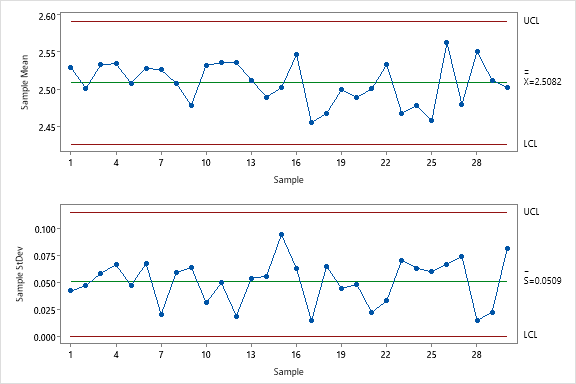
\includegraphics[width=0.75\textwidth]{Xbar_S_Paper.png}
\end{figure}


\item Una empresa que fabrica tarjetas de circuitos impresos desea evaluar si la implementaci\'on de un nuevo sistema de ensamblaje ha reducido el n\'umero de disconformidades. Se tomaron 50 mediciones, antes y después del cambio, para analizar los efectos.
\begin{center}
\begin{tabular}{|l|c|c|}
\hline
 & Antes & Después \\ 
\hline
Media muestral & 3.60 & 2.37 \\ 
\hline
Desviaci'on est'andar muestral & 1.09 & 1.62 \\ 
\hline
\end{tabular}
\end{center}
\begin{enumerate}
\item (15 pts) Calcula un intervalo de confianza de 90\% para el número medio de disconformidades antes del cambio.
\item (15 pts) Calcula un intervalo de confianza de 90\% para la estimar la diferencia en el número medio de disconformidades antes y después del cambio. ¿Qu\'e puedes concluir con este resultado?
\end{enumerate}


\end{enumerate}
  
\newpage



\begin{center}
{\large Instituto Tecnol\'{o}gico y de Estudios Superiores de Monterrey \\
An\'alisis Estad\'stico de Datos } \\
Examen Argumentativo (Papel)
\end{center}

Nombre: \underline{\hspace*{.2in}}
Adriana Molina Gonz\'alez
\underline{\hspace*{.2in}} \quad Matr\'icula:\underline{\hspace*{.2in}}
A01741552
\underline{\hspace*{.2in}} \\

{\bf Instrucciones:} Lee con cuidado cada problema y escribe la soluci\'on
en tu hoja de respuesta. Incluye tu procedimiento que muestre c\'omo obtienes tu respuesta.  Respeta el c\'odigo de \'etica del curso y del Tecnol\'ogico de Monterrey y responde los ejercicios de manera individual sin ayuda externa o no autorizada.

\begin{enumerate}

\item Una empresa que fabrica l\'aminas de aluminio para la industria aeron\'autica necesita asegurar que el espesor de sus l\'aminas cumple con las especificaciones de $2.5 \pm 0.1$ mm. Se ha implementado una nueva maquinaria y se desea monitorear el espesor de las l\'aminas. Para ello, se han tomado muestras de tama\~no 4 cada hora y se gener\'o el diagrama que se muestra abajo.
\begin{enumerate}
\item (5 pts) Calcula la media y variabilidad del proceso (dentro de grupos).
\item (10 pts) Calcula los l\'imites de control para la {\bf variabilidad} del espesor de las láminas.
\item (10 pts) Calcula el porcentaje de l\'aminas que tienen un espesor mayor a 2.6 mm. Use los valores del inciso a) para calcular este porcentaje.
\end{enumerate}
\begin{figure}[h!]
\centering
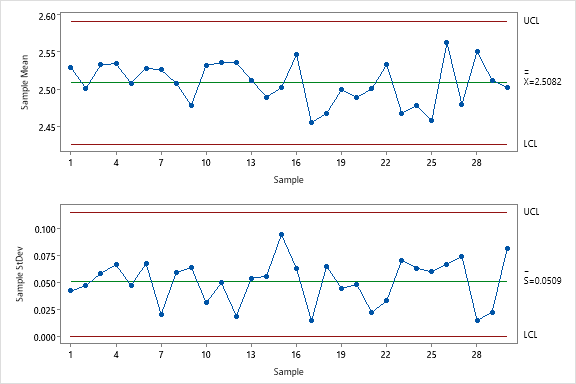
\includegraphics[width=0.75\textwidth]{Xbar_S_Paper.png}
\end{figure}


\item Una empresa que fabrica tarjetas de circuitos impresos desea evaluar si la implementaci\'on de un nuevo sistema de ensamblaje ha reducido el n\'umero de disconformidades. Se tomaron 50 mediciones, antes y después del cambio, para analizar los efectos.
\begin{center}
\begin{tabular}{|l|c|c|}
\hline
 & Antes & Después \\ 
\hline
Media muestral & 3.60 & 2.37 \\ 
\hline
Desviaci'on est'andar muestral & 1.09 & 1.62 \\ 
\hline
\end{tabular}
\end{center}
\begin{enumerate}
\item (15 pts) Calcula un intervalo de confianza de 90\% para el número medio de disconformidades antes del cambio.
\item (15 pts) Calcula un intervalo de confianza de 90\% para la estimar la diferencia en el número medio de disconformidades antes y después del cambio. ¿Qu\'e puedes concluir con este resultado?
\end{enumerate}


\end{enumerate}
  
\newpage



\begin{center}
{\large Instituto Tecnol\'{o}gico y de Estudios Superiores de Monterrey \\
An\'alisis Estad\'stico de Datos } \\
Examen Argumentativo (Papel)
\end{center}

Nombre: \underline{\hspace*{.2in}}
Jorge Sebasti\'an Padilla Duarte
\underline{\hspace*{.2in}} \quad Matr\'icula:\underline{\hspace*{.2in}}
A01743267
\underline{\hspace*{.2in}} \\

{\bf Instrucciones:} Lee con cuidado cada problema y escribe la soluci\'on
en tu hoja de respuesta. Incluye tu procedimiento que muestre c\'omo obtienes tu respuesta.  Respeta el c\'odigo de \'etica del curso y del Tecnol\'ogico de Monterrey y responde los ejercicios de manera individual sin ayuda externa o no autorizada.

\begin{enumerate}

\item Una empresa que fabrica l\'aminas de aluminio para la industria aeron\'autica necesita asegurar que el espesor de sus l\'aminas cumple con las especificaciones de $2.5 \pm 0.1$ mm. Se ha implementado una nueva maquinaria y se desea monitorear el espesor de las l\'aminas. Para ello, se han tomado muestras de tama\~no 4 cada hora y se gener\'o el diagrama que se muestra abajo.
\begin{enumerate}
\item (5 pts) Calcula la media y variabilidad del proceso (dentro de grupos).
\item (10 pts) Calcula los l\'imites de control para el espesor de las láminas.
\item (10 pts) Calcula el porcentaje de l\'aminas que cumplen con las especificaciones. Use los valores del inciso a) para calcular este porcentaje.
\end{enumerate}
\begin{figure}[h!]
\centering
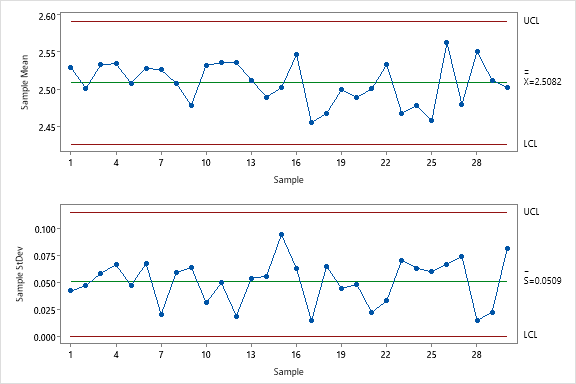
\includegraphics[width=0.75\textwidth]{Xbar_S_Paper.png}
\end{figure}


\item Una empresa que fabrica tarjetas de circuitos impresos desea evaluar si la implementaci\'on de un nuevo sistema de ensamblaje ha reducido el n\'umero de disconformidades. Se tomaron 50 mediciones, antes y después del cambio, para analizar los efectos.
\begin{center}
\begin{tabular}{|l|c|c|}
\hline
 & Antes & Después \\ 
\hline
Media muestral & 3.60 & 2.37 \\ 
\hline
Desviaci'on est'andar muestral & 1.09 & 1.62 \\ 
\hline
\end{tabular}
\end{center}
\begin{enumerate}
\item (15 pts) Calcula un intervalo de confianza de 90\% para el número medio de disconformidades antes del cambio.
\item (15 pts) Calcula un intervalo de confianza de 90\% para la estimar la diferencia en el número medio de disconformidades antes y después del cambio. ¿Qu\'e puedes concluir con este resultado?
\end{enumerate}


\end{enumerate}
  
\newpage



\begin{center}
{\large Instituto Tecnol\'{o}gico y de Estudios Superiores de Monterrey \\
An\'alisis Estad\'stico de Datos } \\
Examen Argumentativo (Papel)
\end{center}

Nombre: \underline{\hspace*{.2in}}
Anna Karenina Reyes Garc\'ia
\underline{\hspace*{.2in}} \quad Matr\'icula:\underline{\hspace*{.2in}}
A01742810
\underline{\hspace*{.2in}} \\

{\bf Instrucciones:} Lee con cuidado cada problema y escribe la soluci\'on
en tu hoja de respuesta. Incluye tu procedimiento que muestre c\'omo obtienes tu respuesta.  Respeta el c\'odigo de \'etica del curso y del Tecnol\'ogico de Monterrey y responde los ejercicios de manera individual sin ayuda externa o no autorizada.

\begin{enumerate}

\item Una empresa que fabrica l\'aminas de aluminio para la industria aeron\'autica necesita asegurar que el espesor de sus l\'aminas cumple con las especificaciones de $2.5 \pm 0.1$ mm. Se ha implementado una nueva maquinaria y se desea monitorear el espesor de las l\'aminas. Para ello, se han tomado muestras de tama\~no 5 cada hora y se gener\'o el diagrama que se muestra abajo.
\begin{enumerate}
\item (5 pts) Calcula la media y variabilidad del proceso (dentro de grupos).
\item (10 pts) Calcula los l\'imites de control para el espesor de las láminas.
\item (10 pts) Calcula el porcentaje de l\'aminas que no cumplen con las especificaciones. Use los valores del inciso a) para calcular este porcentaje.
\end{enumerate}
\begin{figure}[h!]
\centering
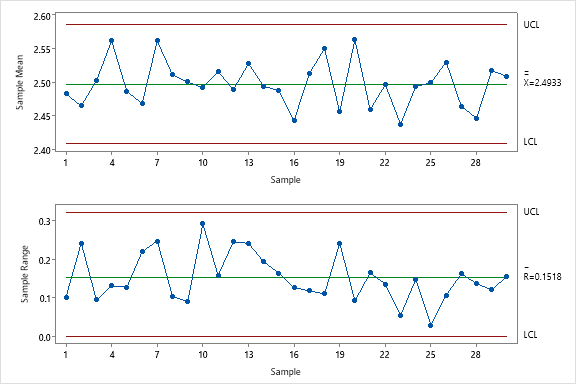
\includegraphics[width=0.75\textwidth]{Xbar_R_Paper.png}
\end{figure}


\item Una empresa que fabrica tarjetas de circuitos impresos desea evaluar si la implementaci\'on de un nuevo sistema de ensamblaje ha reducido el n\'umero de disconformidades. Se tomaron 50 mediciones, antes y después del cambio, para analizar los efectos.
\begin{center}
\begin{tabular}{|l|c|c|}
\hline
 & Antes & Después \\ 
\hline
Media muestral & 3.60 & 2.37 \\ 
\hline
Desviaci'on est'andar muestral & 1.09 & 1.62 \\ 
\hline
\end{tabular}
\end{center}
\begin{enumerate}
\item (15 pts) Calcula un intervalo de confianza de 90\% para el número medio de disconformidades antes del cambio.
\item (15 pts) ¿Existe suficiente evidencia para concluir que el número medio de disconformidades ha disminuido despu\'es del cambio? Usa un nivel de significancia de 0.05.
\end{enumerate}


\end{enumerate}
  
\newpage



\begin{center}
{\large Instituto Tecnol\'{o}gico y de Estudios Superiores de Monterrey \\
An\'alisis Estad\'stico de Datos } \\
Examen Argumentativo (Papel)
\end{center}

Nombre: \underline{\hspace*{.2in}}
Sof\'ia Reyes Meza
\underline{\hspace*{.2in}} \quad Matr\'icula:\underline{\hspace*{.2in}}
A01741675
\underline{\hspace*{.2in}} \\

{\bf Instrucciones:} Lee con cuidado cada problema y escribe la soluci\'on
en tu hoja de respuesta. Incluye tu procedimiento que muestre c\'omo obtienes tu respuesta.  Respeta el c\'odigo de \'etica del curso y del Tecnol\'ogico de Monterrey y responde los ejercicios de manera individual sin ayuda externa o no autorizada.

\begin{enumerate}

\item Una empresa que fabrica l\'aminas de aluminio para la industria aeron\'autica necesita asegurar que el espesor de sus l\'aminas cumple con las especificaciones de $2.5 \pm 0.1$ mm. Se ha implementado una nueva maquinaria y se desea monitorear el espesor de las l\'aminas. Para ello, se han tomado muestras de tama\~no 4 cada hora y se gener\'o el diagrama que se muestra abajo.
\begin{enumerate}
\item (5 pts) Calcula la media y variabilidad del proceso (dentro de grupos).
\item (10 pts) Calcula los l\'imites de control para la {\bf variabilidad} del espesor de las láminas.
\item (10 pts) Calcula el porcentaje de l\'aminas que tienen un espesor mayor a 2.6 mm. Use los valores del inciso a) para calcular este porcentaje.
\end{enumerate}
\begin{figure}[h!]
\centering
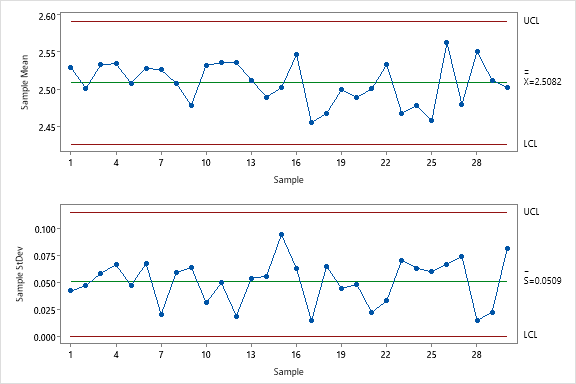
\includegraphics[width=0.75\textwidth]{Xbar_S_Paper.png}
\end{figure}


\item Una empresa que fabrica tarjetas de circuitos impresos desea evaluar si la implementaci\'on de un nuevo sistema de ensamblaje ha reducido el n\'umero de disconformidades. Se tomaron 50 mediciones, antes y después del cambio, para analizar los efectos.
\begin{center}
\begin{tabular}{|l|c|c|}
\hline
 & Antes & Después \\ 
\hline
Media muestral & 3.60 & 2.37 \\ 
\hline
Desviaci'on est'andar muestral & 1.09 & 1.62 \\ 
\hline
\end{tabular}
\end{center}
\begin{enumerate}
\item (15 pts) Calcula un intervalo de confianza de 90\% para el número medio de disconformidades antes del cambio.
\item (15 pts) Calcula un intervalo de confianza de 90\% para la estimar la diferencia en el número medio de disconformidades antes y después del cambio. ¿Qu\'e puedes concluir con este resultado?
\end{enumerate}


\end{enumerate}
  
\newpage



\begin{center}
{\large Instituto Tecnol\'{o}gico y de Estudios Superiores de Monterrey \\
An\'alisis Estad\'stico de Datos } \\
Examen Argumentativo (Papel)
\end{center}

Nombre: \underline{\hspace*{.2in}}
Mar\'ia Jos\'e Rivera Avitia
\underline{\hspace*{.2in}} \quad Matr\'icula:\underline{\hspace*{.2in}}
A01741724
\underline{\hspace*{.2in}} \\

{\bf Instrucciones:} Lee con cuidado cada problema y escribe la soluci\'on
en tu hoja de respuesta. Incluye tu procedimiento que muestre c\'omo obtienes tu respuesta.  Respeta el c\'odigo de \'etica del curso y del Tecnol\'ogico de Monterrey y responde los ejercicios de manera individual sin ayuda externa o no autorizada.

\begin{enumerate}

\item Una empresa que fabrica l\'aminas de aluminio para la industria aeron\'autica necesita asegurar que el espesor de sus l\'aminas cumple con las especificaciones de $2.5 \pm 0.1$ mm. Se ha implementado una nueva maquinaria y se desea monitorear el espesor de las l\'aminas. Para ello, se han tomado muestras de tama\~no 5 cada hora y se gener\'o el diagrama que se muestra abajo.
\begin{enumerate}
\item (5 pts) Calcula la media y variabilidad del proceso (dentro de grupos).
\item (10 pts) Calcula los l\'imites de control para el espesor de las láminas.
\item (10 pts) Calcula el porcentaje de l\'aminas que no cumplen con las especificaciones. Use los valores del inciso a) para calcular este porcentaje.
\end{enumerate}
\begin{figure}[h!]
\centering
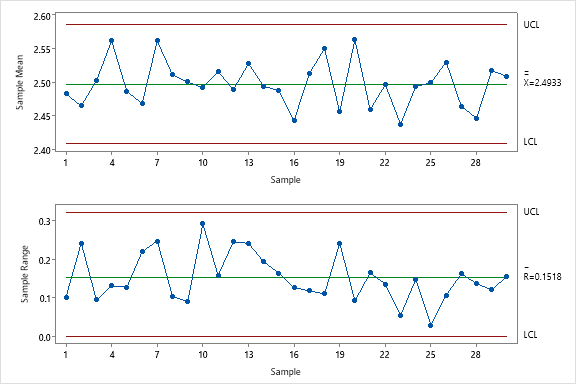
\includegraphics[width=0.75\textwidth]{Xbar_R_Paper.png}
\end{figure}


\item Una empresa que fabrica tarjetas de circuitos impresos desea evaluar si la implementaci\'on de un nuevo sistema de ensamblaje ha reducido el n\'umero de disconformidades. Se tomaron 50 mediciones, antes y después del cambio, para analizar los efectos.
\begin{center}
\begin{tabular}{|l|c|c|}
\hline
 & Antes & Después \\ 
\hline
Media muestral & 3.60 & 2.37 \\ 
\hline
Desviaci'on est'andar muestral & 1.09 & 1.62 \\ 
\hline
\end{tabular}
\end{center}
\begin{enumerate}
\item (15 pts) Calcula un intervalo de confianza de 90\% para el número medio de disconformidades antes del cambio.
\item (15 pts) Calcula un intervalo de confianza de 90\% para la estimar la diferencia en el número medio de disconformidades antes y después del cambio. ¿Qu\'e puedes concluir con este resultado?
\end{enumerate}


\end{enumerate}
  
\newpage



\begin{center}
{\large Instituto Tecnol\'{o}gico y de Estudios Superiores de Monterrey \\
An\'alisis Estad\'stico de Datos } \\
Examen Argumentativo (Papel)
\end{center}

Nombre: \underline{\hspace*{.2in}}
Carlo Santiago S\'anchez Beltr\'an
\underline{\hspace*{.2in}} \quad Matr\'icula:\underline{\hspace*{.2in}}
A01743074
\underline{\hspace*{.2in}} \\

{\bf Instrucciones:} Lee con cuidado cada problema y escribe la soluci\'on
en tu hoja de respuesta. Incluye tu procedimiento que muestre c\'omo obtienes tu respuesta.  Respeta el c\'odigo de \'etica del curso y del Tecnol\'ogico de Monterrey y responde los ejercicios de manera individual sin ayuda externa o no autorizada.

\begin{enumerate}

\item Una empresa que fabrica l\'aminas de aluminio para la industria aeron\'autica necesita asegurar que el espesor de sus l\'aminas cumple con las especificaciones de $2.5 \pm 0.1$ mm. Se ha implementado una nueva maquinaria y se desea monitorear el espesor de las l\'aminas. Para ello, se han tomado muestras de tama\~no 4 cada hora y se gener\'o el diagrama que se muestra abajo.
\begin{enumerate}
\item (5 pts) Calcula la media y variabilidad del proceso (dentro de grupos).
\item (10 pts) Calcula los l\'imites de control para la {\bf variabilidad} del espesor de las láminas.
\item (10 pts) Calcula el porcentaje de l\'aminas que tienen un espesor mayor a 2.6 mm. Use los valores del inciso a) para calcular este porcentaje.
\end{enumerate}
\begin{figure}[h!]
\centering
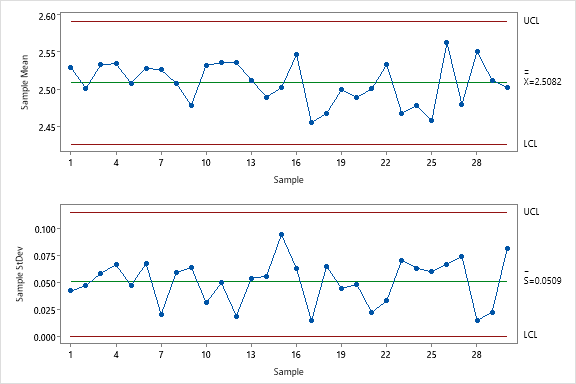
\includegraphics[width=0.75\textwidth]{Xbar_S_Paper.png}
\end{figure}


\item Una empresa que fabrica tarjetas de circuitos impresos desea evaluar si la implementaci\'on de un nuevo sistema de ensamblaje ha reducido el n\'umero de disconformidades. Se tomaron 50 mediciones, antes y después del cambio, para analizar los efectos.
\begin{center}
\begin{tabular}{|l|c|c|}
\hline
 & Antes & Después \\ 
\hline
Media muestral & 3.60 & 2.37 \\ 
\hline
Desviaci'on est'andar muestral & 1.09 & 1.62 \\ 
\hline
\end{tabular}
\end{center}
\begin{enumerate}
\item (15 pts) Calcula un intervalo de confianza de 90\% para el número medio de disconformidades antes del cambio.
\item (15 pts) ¿Existe suficiente evidencia para concluir que el número medio de disconformidades ha disminuido despu\'es del cambio? Usa un nivel de significancia de 0.05.
\end{enumerate}


\end{enumerate}
  
\newpage



\begin{center}
{\large Instituto Tecnol\'{o}gico y de Estudios Superiores de Monterrey \\
An\'alisis Estad\'stico de Datos } \\
Examen Argumentativo (Papel)
\end{center}

Nombre: \underline{\hspace*{.2in}}
Pedro Anibal Santiago Molina
\underline{\hspace*{.2in}} \quad Matr\'icula:\underline{\hspace*{.2in}}
A01743251
\underline{\hspace*{.2in}} \\

{\bf Instrucciones:} Lee con cuidado cada problema y escribe la soluci\'on
en tu hoja de respuesta. Incluye tu procedimiento que muestre c\'omo obtienes tu respuesta.  Respeta el c\'odigo de \'etica del curso y del Tecnol\'ogico de Monterrey y responde los ejercicios de manera individual sin ayuda externa o no autorizada.

\begin{enumerate}

\item Una empresa que fabrica l\'aminas de aluminio para la industria aeron\'autica necesita asegurar que el espesor de sus l\'aminas cumple con las especificaciones de $2.5 \pm 0.1$ mm. Se ha implementado una nueva maquinaria y se desea monitorear el espesor de las l\'aminas. Para ello, se han tomado muestras de tama\~no 4 cada hora y se gener\'o el diagrama que se muestra abajo.
\begin{enumerate}
\item (5 pts) Calcula la media y variabilidad del proceso (dentro de grupos).
\item (10 pts) Calcula los l\'imites de control para el espesor de las láminas.
\item (10 pts) Calcula el porcentaje de l\'aminas que cumplen con las especificaciones. Use los valores del inciso a) para calcular este porcentaje.
\end{enumerate}
\begin{figure}[h!]
\centering
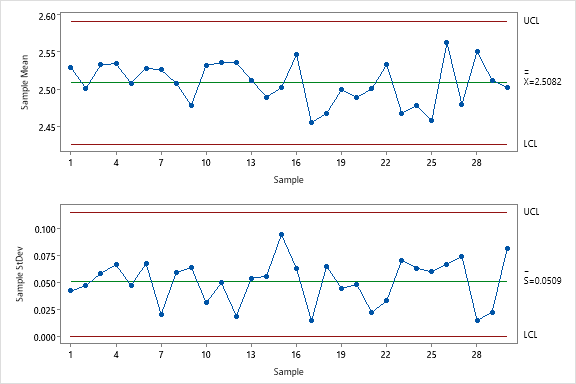
\includegraphics[width=0.75\textwidth]{Xbar_S_Paper.png}
\end{figure}


\item Una empresa que fabrica tarjetas de circuitos impresos desea evaluar si la implementaci\'on de un nuevo sistema de ensamblaje ha reducido el n\'umero de disconformidades. Se tomaron 50 mediciones, antes y después del cambio, para analizar los efectos.
\begin{center}
\begin{tabular}{|l|c|c|}
\hline
 & Antes & Después \\ 
\hline
Media muestral & 3.60 & 2.37 \\ 
\hline
Desviaci'on est'andar muestral & 1.09 & 1.62 \\ 
\hline
\end{tabular}
\end{center}
\begin{enumerate}
\item (15 pts) Calcula un intervalo de confianza de 90\% para el número medio de disconformidades antes del cambio.
\item (15 pts) ¿Existe suficiente evidencia para concluir que el número medio de disconformidades ha disminuido despu\'es del cambio? Usa un nivel de significancia de 0.05.
\end{enumerate}


\end{enumerate}
  
\newpage



\begin{center}
{\large Instituto Tecnol\'{o}gico y de Estudios Superiores de Monterrey \\
An\'alisis Estad\'stico de Datos } \\
Examen Argumentativo (Papel)
\end{center}

Nombre: \underline{\hspace*{.2in}}
Ana Sof\'ia Soltero Am\'ezquita
\underline{\hspace*{.2in}} \quad Matr\'icula:\underline{\hspace*{.2in}}
A01741188
\underline{\hspace*{.2in}} \\

{\bf Instrucciones:} Lee con cuidado cada problema y escribe la soluci\'on
en tu hoja de respuesta. Incluye tu procedimiento que muestre c\'omo obtienes tu respuesta.  Respeta el c\'odigo de \'etica del curso y del Tecnol\'ogico de Monterrey y responde los ejercicios de manera individual sin ayuda externa o no autorizada.

\begin{enumerate}

\item Una empresa que fabrica l\'aminas de aluminio para la industria aeron\'autica necesita asegurar que el espesor de sus l\'aminas cumple con las especificaciones de $2.5 \pm 0.1$ mm. Se ha implementado una nueva maquinaria y se desea monitorear el espesor de las l\'aminas. Para ello, se han tomado muestras de tama\~no 4 cada hora y se gener\'o el diagrama que se muestra abajo.
\begin{enumerate}
\item (5 pts) Calcula la media y variabilidad del proceso (dentro de grupos).
\item (10 pts) Calcula los l\'imites de control para la {\bf variabilidad} del espesor de las láminas.
\item (10 pts) Calcula el porcentaje de l\'aminas que tienen un espesor mayor a 2.6 mm. Use los valores del inciso a) para calcular este porcentaje.
\end{enumerate}
\begin{figure}[h!]
\centering
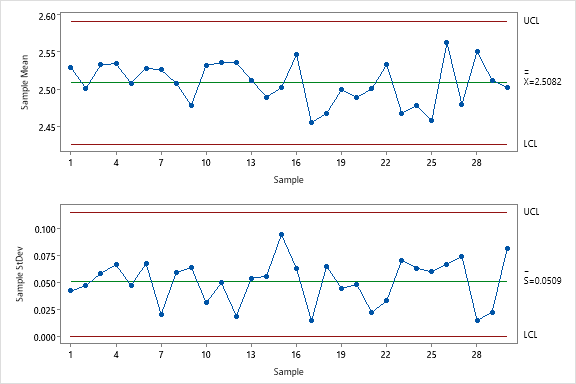
\includegraphics[width=0.75\textwidth]{Xbar_S_Paper.png}
\end{figure}


\item Una empresa que fabrica tarjetas de circuitos impresos desea evaluar si la implementaci\'on de un nuevo sistema de ensamblaje ha reducido el n\'umero de disconformidades. Se tomaron 50 mediciones, antes y después del cambio, para analizar los efectos.
\begin{center}
\begin{tabular}{|l|c|c|}
\hline
 & Antes & Después \\ 
\hline
Media muestral & 3.60 & 2.37 \\ 
\hline
Desviaci'on est'andar muestral & 1.09 & 1.62 \\ 
\hline
\end{tabular}
\end{center}
\begin{enumerate}
\item (15 pts) Calcula un intervalo de confianza de 90\% para el número medio de disconformidades antes del cambio.
\item (15 pts) ¿Existe suficiente evidencia para concluir que el número medio de disconformidades ha disminuido despu\'es del cambio? Usa un nivel de significancia de 0.05.
\end{enumerate}


\end{enumerate}
  
\newpage



\begin{center}
{\large Instituto Tecnol\'{o}gico y de Estudios Superiores de Monterrey \\
An\'alisis Estad\'stico de Datos } \\
Examen Argumentativo (Papel)
\end{center}

Nombre: \underline{\hspace*{.2in}}
Monserrat Soto Palazuelos
\underline{\hspace*{.2in}} \quad Matr\'icula:\underline{\hspace*{.2in}}
A01741648
\underline{\hspace*{.2in}} \\

{\bf Instrucciones:} Lee con cuidado cada problema y escribe la soluci\'on
en tu hoja de respuesta. Incluye tu procedimiento que muestre c\'omo obtienes tu respuesta.  Respeta el c\'odigo de \'etica del curso y del Tecnol\'ogico de Monterrey y responde los ejercicios de manera individual sin ayuda externa o no autorizada.

\begin{enumerate}

\item Una empresa que fabrica l\'aminas de aluminio para la industria aeron\'autica necesita asegurar que el espesor de sus l\'aminas cumple con las especificaciones de $2.5 \pm 0.1$ mm. Se ha implementado una nueva maquinaria y se desea monitorear el espesor de las l\'aminas. Para ello, se han tomado muestras de tama\~no 4 cada hora y se gener\'o el diagrama que se muestra abajo.
\begin{enumerate}
\item (5 pts) Calcula la media y variabilidad del proceso (dentro de grupos).
\item (10 pts) Calcula los l\'imites de control para la {\bf variabilidad} del espesor de las láminas.
\item (10 pts) Calcula el porcentaje de l\'aminas que tienen un espesor mayor a 2.6 mm. Use los valores del inciso a) para calcular este porcentaje.
\end{enumerate}
\begin{figure}[h!]
\centering
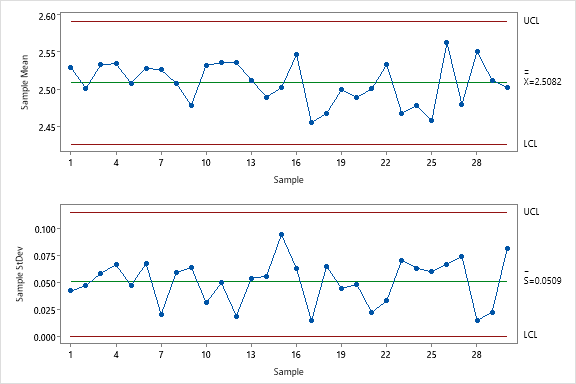
\includegraphics[width=0.75\textwidth]{Xbar_S_Paper.png}
\end{figure}


\item Una empresa que fabrica tarjetas de circuitos impresos desea evaluar si la implementaci\'on de un nuevo sistema de ensamblaje ha reducido el n\'umero de disconformidades. Se tomaron 50 mediciones, antes y después del cambio, para analizar los efectos.
\begin{center}
\begin{tabular}{|l|c|c|}
\hline
 & Antes & Después \\ 
\hline
Media muestral & 3.60 & 2.37 \\ 
\hline
Desviaci'on est'andar muestral & 1.09 & 1.62 \\ 
\hline
\end{tabular}
\end{center}
\begin{enumerate}
\item (15 pts) Calcula un intervalo de confianza de 90\% para el número medio de disconformidades antes del cambio.
\item (15 pts) ¿Existe suficiente evidencia para concluir que el número medio de disconformidades ha disminuido despu\'es del cambio? Usa un nivel de significancia de 0.05.
\end{enumerate}


\end{enumerate}
  
\newpage



\begin{center}
{\large Instituto Tecnol\'{o}gico y de Estudios Superiores de Monterrey \\
An\'alisis Estad\'stico de Datos } \\
Examen Argumentativo (Papel)
\end{center}

Nombre: \underline{\hspace*{.2in}}
Valeria Tirado Rojo
\underline{\hspace*{.2in}} \quad Matr\'icula:\underline{\hspace*{.2in}}
A01741679
\underline{\hspace*{.2in}} \\

{\bf Instrucciones:} Lee con cuidado cada problema y escribe la soluci\'on
en tu hoja de respuesta. Incluye tu procedimiento que muestre c\'omo obtienes tu respuesta.  Respeta el c\'odigo de \'etica del curso y del Tecnol\'ogico de Monterrey y responde los ejercicios de manera individual sin ayuda externa o no autorizada.

\begin{enumerate}

\item Una empresa que fabrica l\'aminas de aluminio para la industria aeron\'autica necesita asegurar que el espesor de sus l\'aminas cumple con las especificaciones de $2.5 \pm 0.1$ mm. Se ha implementado una nueva maquinaria y se desea monitorear el espesor de las l\'aminas. Para ello, se han tomado muestras de tama\~no 4 cada hora y se gener\'o el diagrama que se muestra abajo.
\begin{enumerate}
\item (5 pts) Calcula la media y variabilidad del proceso (dentro de grupos).
\item (10 pts) Calcula los l\'imites de control para la {\bf variabilidad} del espesor de las láminas.
\item (10 pts) Calcula el porcentaje de l\'aminas que tienen un espesor mayor a 2.6 mm. Use los valores del inciso a) para calcular este porcentaje.
\end{enumerate}
\begin{figure}[h!]
\centering
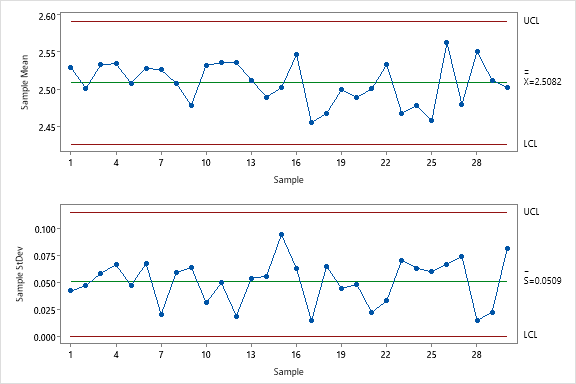
\includegraphics[width=0.75\textwidth]{Xbar_S_Paper.png}
\end{figure}


\item Una empresa que fabrica tarjetas de circuitos impresos desea evaluar si la implementaci\'on de un nuevo sistema de ensamblaje ha reducido el n\'umero de disconformidades. Se tomaron 50 mediciones, antes y después del cambio, para analizar los efectos.
\begin{center}
\begin{tabular}{|l|c|c|}
\hline
 & Antes & Después \\ 
\hline
Media muestral & 3.60 & 2.37 \\ 
\hline
Desviaci'on est'andar muestral & 1.09 & 1.62 \\ 
\hline
\end{tabular}
\end{center}
\begin{enumerate}
\item (15 pts) Calcula un intervalo de confianza de 90\% para el número medio de disconformidades antes del cambio.
\item (15 pts) ¿Existe suficiente evidencia para concluir que el número medio de disconformidades ha disminuido despu\'es del cambio? Usa un nivel de significancia de 0.05.
\end{enumerate}


\end{enumerate}
  
\newpage



\begin{center}
{\large Instituto Tecnol\'{o}gico y de Estudios Superiores de Monterrey \\
An\'alisis Estad\'stico de Datos } \\
Examen Argumentativo (Papel)
\end{center}

Nombre: \underline{\hspace*{.2in}}
Luis Valenzuela G\'omez
\underline{\hspace*{.2in}} \quad Matr\'icula:\underline{\hspace*{.2in}}
A01741799
\underline{\hspace*{.2in}} \\

{\bf Instrucciones:} Lee con cuidado cada problema y escribe la soluci\'on
en tu hoja de respuesta. Incluye tu procedimiento que muestre c\'omo obtienes tu respuesta.  Respeta el c\'odigo de \'etica del curso y del Tecnol\'ogico de Monterrey y responde los ejercicios de manera individual sin ayuda externa o no autorizada.

\begin{enumerate}

\item Una empresa que fabrica l\'aminas de aluminio para la industria aeron\'autica necesita asegurar que el espesor de sus l\'aminas cumple con las especificaciones de $2.5 \pm 0.1$ mm. Se ha implementado una nueva maquinaria y se desea monitorear el espesor de las l\'aminas. Para ello, se han tomado muestras de tama\~no 4 cada hora y se gener\'o el diagrama que se muestra abajo.
\begin{enumerate}
\item (5 pts) Calcula la media y variabilidad del proceso (dentro de grupos).
\item (10 pts) Calcula los l\'imites de control para el espesor de las láminas.
\item (10 pts) Calcula el porcentaje de l\'aminas que cumplen con las especificaciones. Use los valores del inciso a) para calcular este porcentaje.
\end{enumerate}
\begin{figure}[h!]
\centering
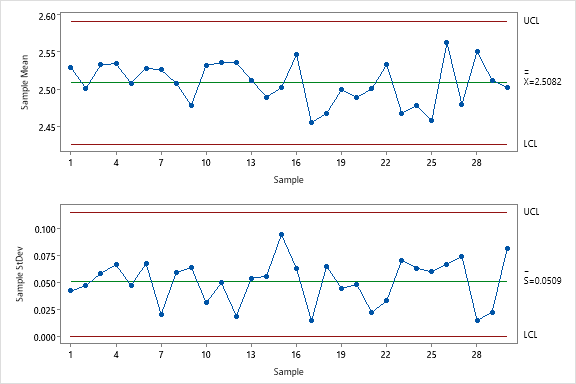
\includegraphics[width=0.75\textwidth]{Xbar_S_Paper.png}
\end{figure}


\item Una empresa que fabrica tarjetas de circuitos impresos desea evaluar si la implementaci\'on de un nuevo sistema de ensamblaje ha reducido el n\'umero de disconformidades. Se tomaron 50 mediciones, antes y después del cambio, para analizar los efectos.
\begin{center}
\begin{tabular}{|l|c|c|}
\hline
 & Antes & Después \\ 
\hline
Media muestral & 3.60 & 2.37 \\ 
\hline
Desviaci'on est'andar muestral & 1.09 & 1.62 \\ 
\hline
\end{tabular}
\end{center}
\begin{enumerate}
\item (15 pts) Calcula un intervalo de confianza de 90\% para el número medio de disconformidades antes del cambio.
\item (15 pts) ¿Existe suficiente evidencia para concluir que el número medio de disconformidades ha disminuido despu\'es del cambio? Usa un nivel de significancia de 0.05.
\end{enumerate}


\end{enumerate}
  
\newpage



\begin{center}
{\large Instituto Tecnol\'{o}gico y de Estudios Superiores de Monterrey \\
An\'alisis Estad\'stico de Datos } \\
Examen Argumentativo (Papel)
\end{center}

Nombre: \underline{\hspace*{.2in}}
Luis Emiliano Villegas Sapiens
\underline{\hspace*{.2in}} \quad Matr\'icula:\underline{\hspace*{.2in}}
A01743220
\underline{\hspace*{.2in}} \\

{\bf Instrucciones:} Lee con cuidado cada problema y escribe la soluci\'on
en tu hoja de respuesta. Incluye tu procedimiento que muestre c\'omo obtienes tu respuesta.  Respeta el c\'odigo de \'etica del curso y del Tecnol\'ogico de Monterrey y responde los ejercicios de manera individual sin ayuda externa o no autorizada.

\begin{enumerate}

\item Una empresa que fabrica l\'aminas de aluminio para la industria aeron\'autica necesita asegurar que el espesor de sus l\'aminas cumple con las especificaciones de $2.5 \pm 0.1$ mm. Se ha implementado una nueva maquinaria y se desea monitorear el espesor de las l\'aminas. Para ello, se han tomado muestras de tama\~no 4 cada hora y se gener\'o el diagrama que se muestra abajo.
\begin{enumerate}
\item (5 pts) Calcula la media y variabilidad del proceso (dentro de grupos).
\item (10 pts) Calcula los l\'imites de control para la {\bf variabilidad} del espesor de las láminas.
\item (10 pts) Calcula el porcentaje de l\'aminas que tienen un espesor mayor a 2.6 mm. Use los valores del inciso a) para calcular este porcentaje.
\end{enumerate}
\begin{figure}[h!]
\centering
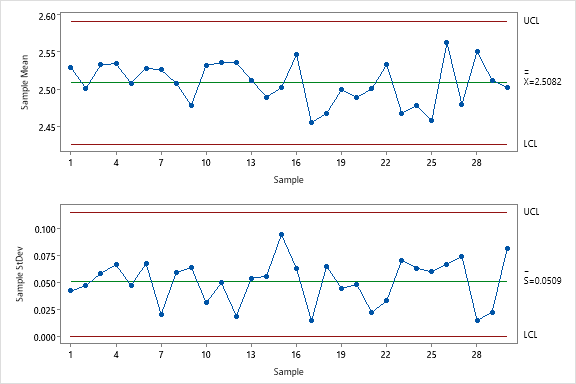
\includegraphics[width=0.75\textwidth]{Xbar_S_Paper.png}
\end{figure}


\item Una empresa que fabrica tarjetas de circuitos impresos desea evaluar si la implementaci\'on de un nuevo sistema de ensamblaje ha reducido el n\'umero de disconformidades. Se tomaron 50 mediciones, antes y después del cambio, para analizar los efectos.
\begin{center}
\begin{tabular}{|l|c|c|}
\hline
 & Antes & Después \\ 
\hline
Media muestral & 3.60 & 2.37 \\ 
\hline
Desviaci'on est'andar muestral & 1.09 & 1.62 \\ 
\hline
\end{tabular}
\end{center}
\begin{enumerate}
\item (15 pts) Calcula un intervalo de confianza de 90\% para el número medio de disconformidades antes del cambio.
\item (15 pts) ¿Existe suficiente evidencia para concluir que el número medio de disconformidades ha disminuido despu\'es del cambio? Usa un nivel de significancia de 0.05.
\end{enumerate}


\end{enumerate}
  
\newpage


\end{document}
